\documentclass[a4paper,11pt,titlepage,uplatex]{jsarticle}

% プリアンブルを外部ファイル化しておきました。中身はmacro.texで確認できます。

\usepackage[dvipdfmx]{graphicx,xcolor}% ドライバ指定
\usepackage[top=30truemm,bottom=30truemm,left=25truemm,right=25truemm]{geometry} % 余白設定

% 画像
\usepackage{here, subfig}
\usepackage{docmute} % ファイル分割用
\usepackage[cc]{titlepic}

% 数式関連
\usepackage{amsmath,amsfonts,amssymb,mathtools,amsthm}
\usepackage{bm} % ボールド体のベクトルを出力するときには\vb{a}ではなく\bm{a}としてください。\bmの方が綺麗に出力できる。
\usepackage{empheq} % 連立方程式をきれいに書いてくれる
\usepackage{physics} % 微分記号とか
\usepackage[separate-uncertainty]{siunitx} % SIUNITX

% 数式、図、表番号の変更
\makeatletter
\@addtoreset{equation}{section} % 章ごとに番号をリセット
\@addtoreset{figure}{section}
\@addtoreset{table}{section}
\def\theequation{\thesection.\arabic{equation}} % 章.何番目 と変更
\def\thefigure{\thesection.\arabic{figure}}
\def\thetable{\thesection.\arabic{table}}
\makeatother

% -------------------
% 定理環境付近
\usepackage{tcolorbox} % 色付きの囲み
\tcbuselibrary{breakable, skins, theorems}
\usepackage{ascmac} % 囲み \begin{itembox}ができる。

% ----------

\usepackage{enumitem} % enumium環境いじるために必要
\renewcommand{\labelenumi}{\theenumi.}
\renewcommand{\theenumi}{\Alph{enumi}}

% ------------ url関係
\usepackage{url}
\usepackage[dvipdfmx]{hyperref}
\hypersetup{
	 colorlinks=true,
	 citecolor=blue,
	 linkcolor=black,
	 urlcolor=blue
}
\usepackage{pxjahyper}
% ---------

% 表関連のパッケージ
\usepackage{booktabs}
\usepackage{multirow}
\usepackage{longtable}
\usepackage{arydshln}% 表で破線を使うため
\usepackage{multicol}
% longtableをusepackageする場合は順番が重要らしいです。longtableとarydshlnの順番逆にしたらエラーはく(コンパイルはできるが…)

\renewcommand{\labelitemii}{・}

\usepackage[greek, japanese]{babel}
\usepackage{teubner}	% 古代(古典)ギリシア語表記指定



% 大槻使用
\usepackage{color}
\newcommand{\red}[1]{\textcolor{red}{#1}}
\newcommand{\blue}[1]{\textcolor{blue}{#1}}
\usepackage{ulem}

% 能崎使用
%背景
\usepackage{wallpaper}

\begin{document}

\section{シミュレーション系}

\subsection{打ち上げ諸元}
\textcolor{red}{絶対ここじゃない}
\begin{table}[H]
    \centering
    \caption{打ち上げに関する諸元}
    \label{tab:utiage_shogen}
    \begin{tabular}{lcr}
        \hline
        名称   & 単位                    & \multicolumn{1}{c}{値} \\
        \hline
        日付   &                       & 2022/11/13            \\
        日時   &                       & 7:47                  \\
        気象   &                       &                       \\
        気温   & \SI{}{\degreeCelsius} & 18.39                 \\
        気圧   & \SI{}{hPa}            & 964.49                \\
        射点高度 & \SI{}{m}              & 430                   \\
        射点緯度 & \SI{}{deg}            & 北緯34.736139           \\
        射点経度 & \SI{}{deg}            & 東経139.421333          \\
        磁気偏向 & \SI{}{deg}            & 7.53(西偏)              \\
        風向   & \SI{}{deg}            & 180                   \\
        風速   & \SI{}{m/s}            & 3.0                   \\
        \hline
    \end{tabular}
\end{table}


\subsection{データ解析}

\subsubsection{位置・速度}
\label{itisokudo}
今回の打ち上げでは、開放基板及びミッション基板それぞれに搭載された6軸センサのロギング及びデータ取得に両者とも成功した。
取得した加速度・角速度センサの値を図\ref{fig:rokuziku}に示す。ただしミッション基板のデータは離床検知後30秒までのものであり、着地前にロギングを終了している。
座標軸に関して、各軸は図に示すとおりである。また、角速度センサについては離床前のデータの平均値を取り、全体から減算する事により0点補正を行っている。

\begin{figure}[H]
    \begin{tabular}{cc}
        \begin{minipage}{.48\textwidth}
            \centering
            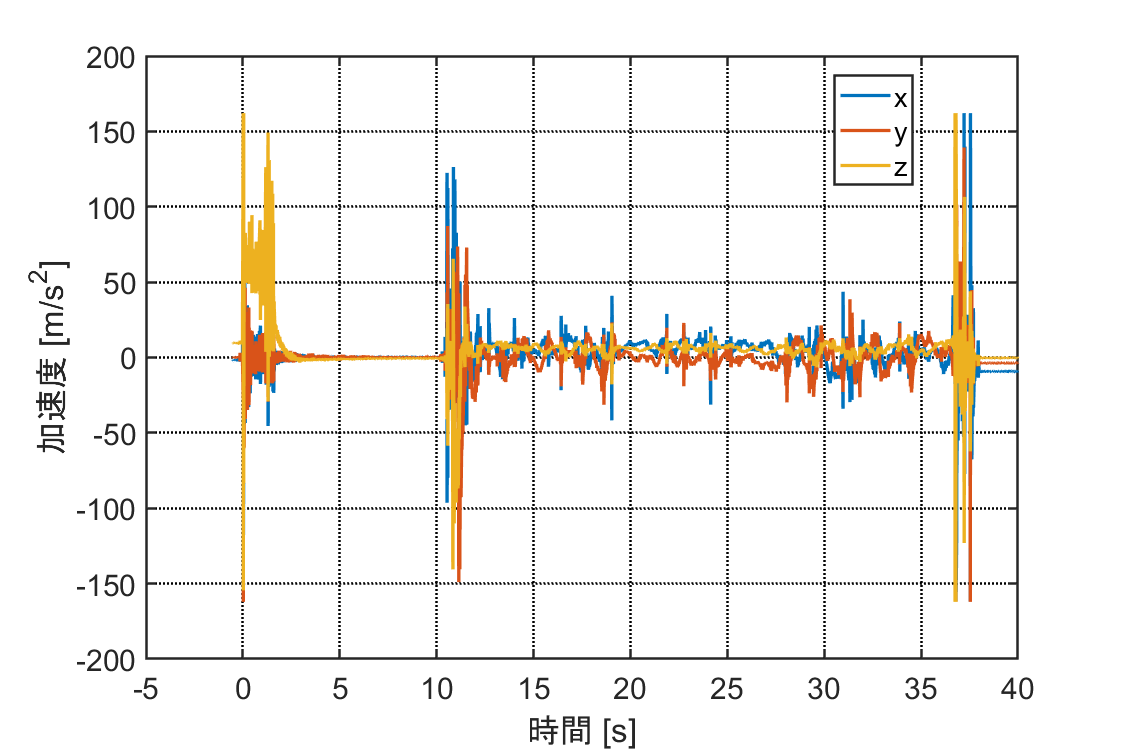
\includegraphics[width=75mm]{pic_sim/acc_no.png}
            \hspace{16mm} {\small[1]加速度データ(開放基板)}
        \end{minipage}
        \begin{minipage}{.48\textwidth}
            \centering
            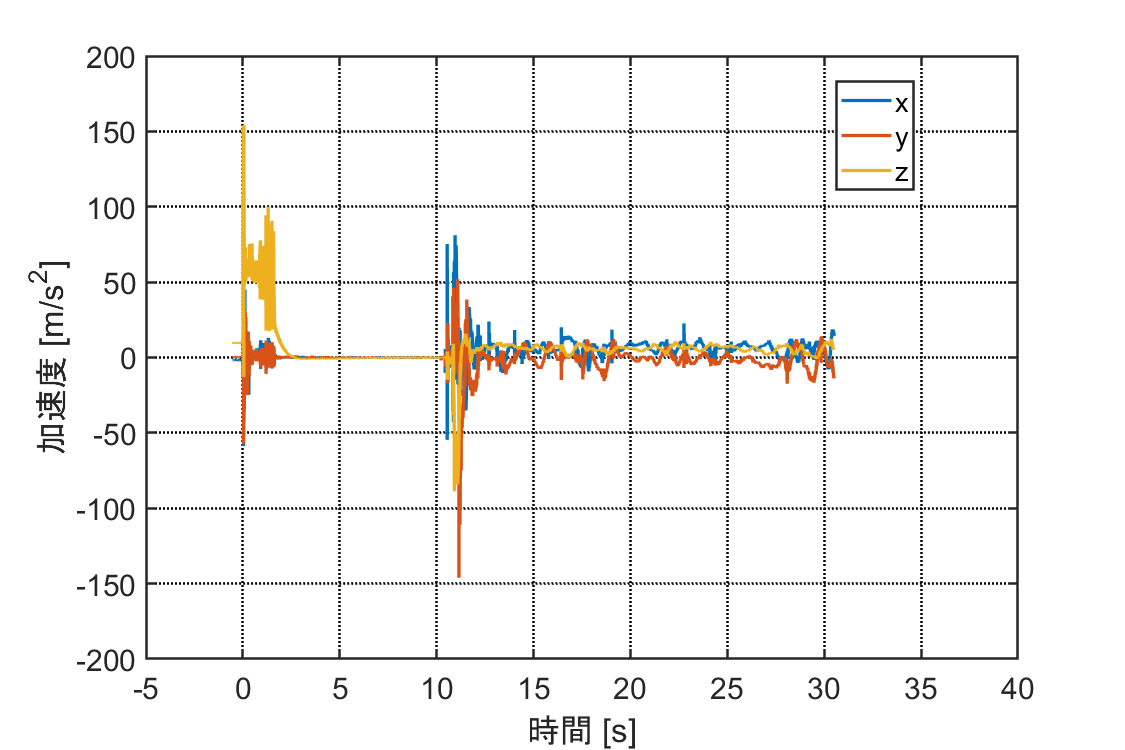
\includegraphics[width=75mm]{pic_sim/acc_ta.png}
            \hspace{16mm} {\small[2]加速度データ(ミッション基板)}
        \end{minipage}
    \end{tabular}
    \begin{tabular}{cc}
        \begin{minipage}{.48\textwidth}
            \centering
            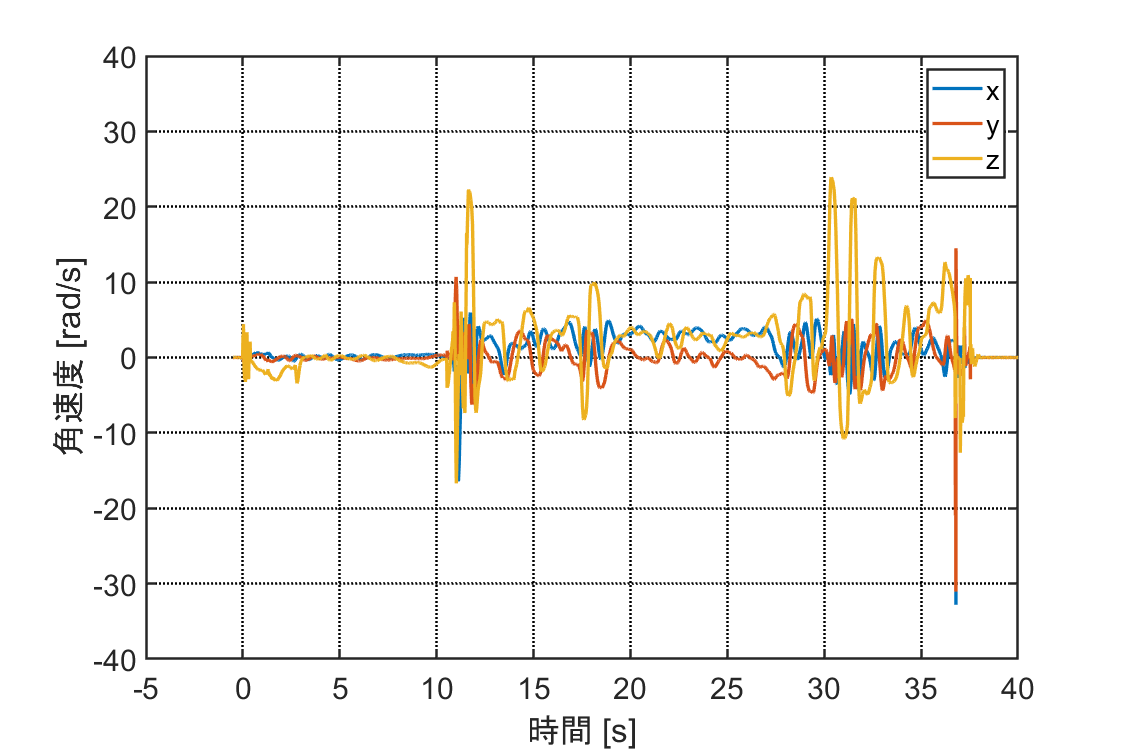
\includegraphics[width=75mm]{pic_sim/gyr_no.png}
            \hspace{16mm} {\small[3]角速度データ(開放基板)}
        \end{minipage}
        \begin{minipage}{.48\textwidth}
            \centering
            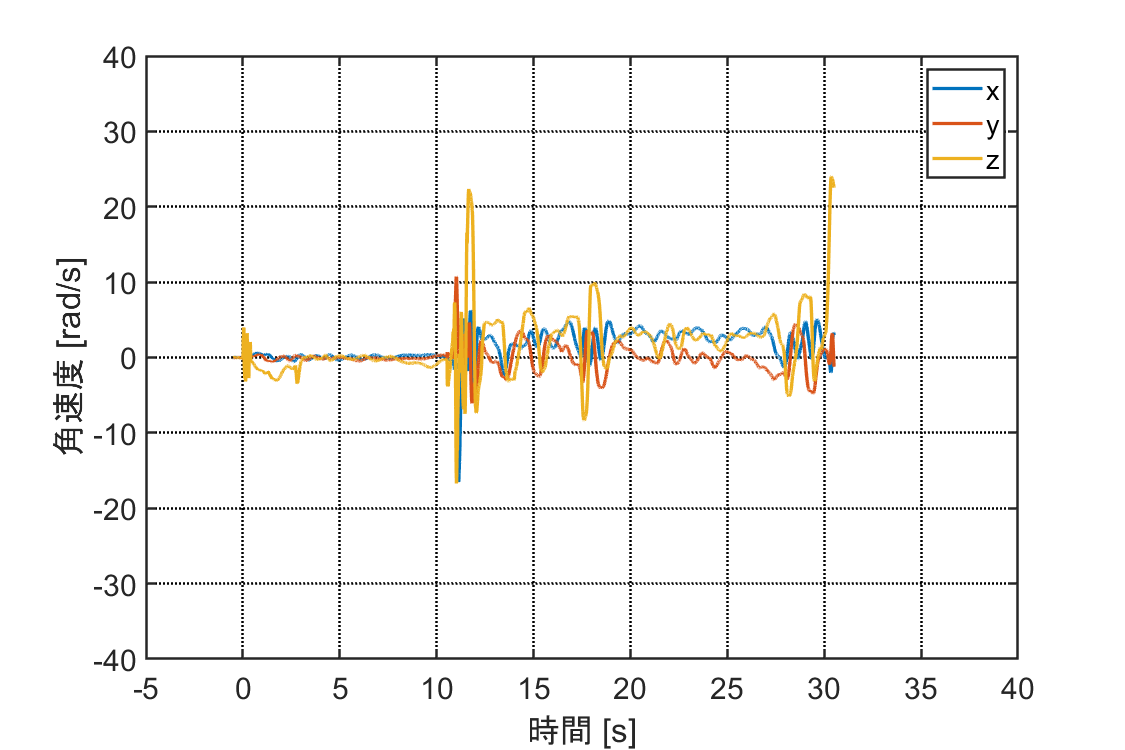
\includegraphics[width=75mm]{pic_sim/gyr_ta.png}
            \hspace{16mm} {\small[4]角速度データ(ミッション基板)}
        \end{minipage}
    \end{tabular}
    \caption{加速度・角速度センサデータ}
    \label{fig:rokuziku}
\end{figure}

取得した加速度・角速度データをもとに積分を行い、対地速度及び飛行経路を算出した。開放基板及びミッション基板それぞれの対地速度を図\ref{fig:taitisokudo}に、算出した飛行経路と実際の着地地点を図\ref{fig:hikoukeiro}に示す。
それぞれの値は射点を原点として磁東を基準としたENU座標系におけるものである。なお、パラシュート開傘以降の6軸センサの積分精度が悪くなることから、パラシュート開放以前は実線、以降は点線としてプロットしている。

\begin{figure}[H]
    \centering
    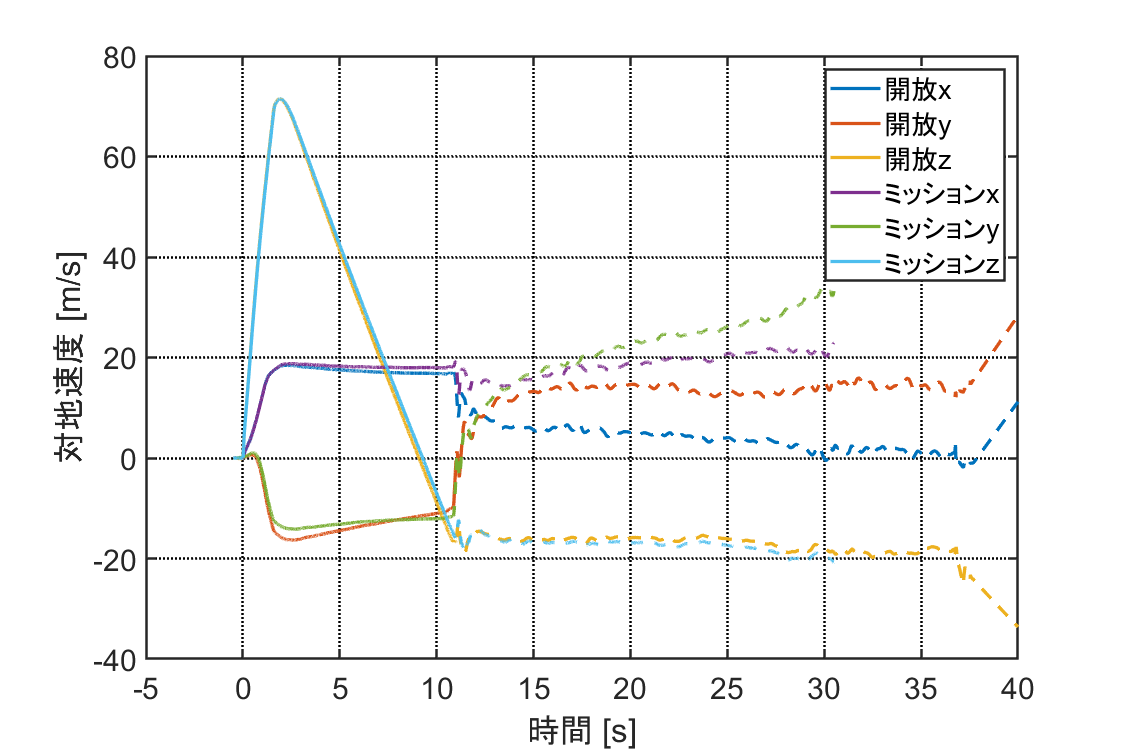
\includegraphics[width=0.7\linewidth]{pic_sim/Ve2.png}
    \caption{対地速度}
    \label{fig:taitisokudo}
\end{figure}

\begin{figure}[H]
    \begin{tabular}{cc}
        \begin{minipage}{.48\textwidth}
            \centering
            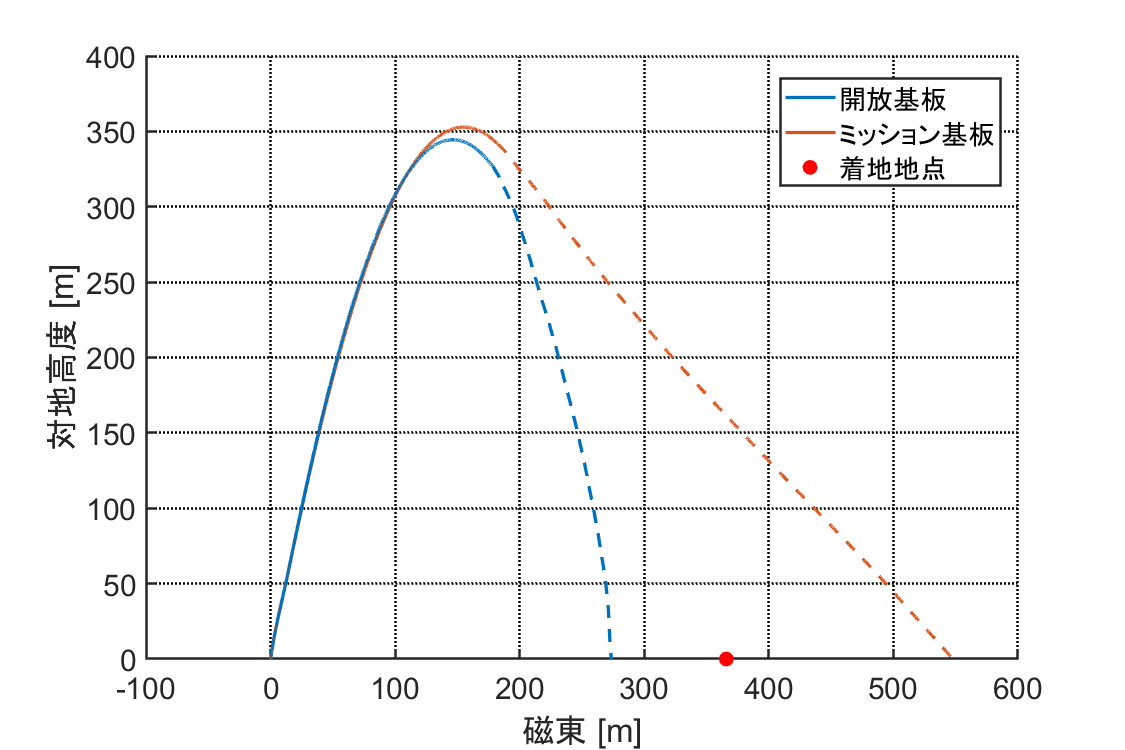
\includegraphics[width=75mm]{pic_sim/pos2_eh.png}
            \hspace{16mm} {\small[1]磁東-対地高度}
        \end{minipage}
        \begin{minipage}{.48\textwidth}
            \centering
            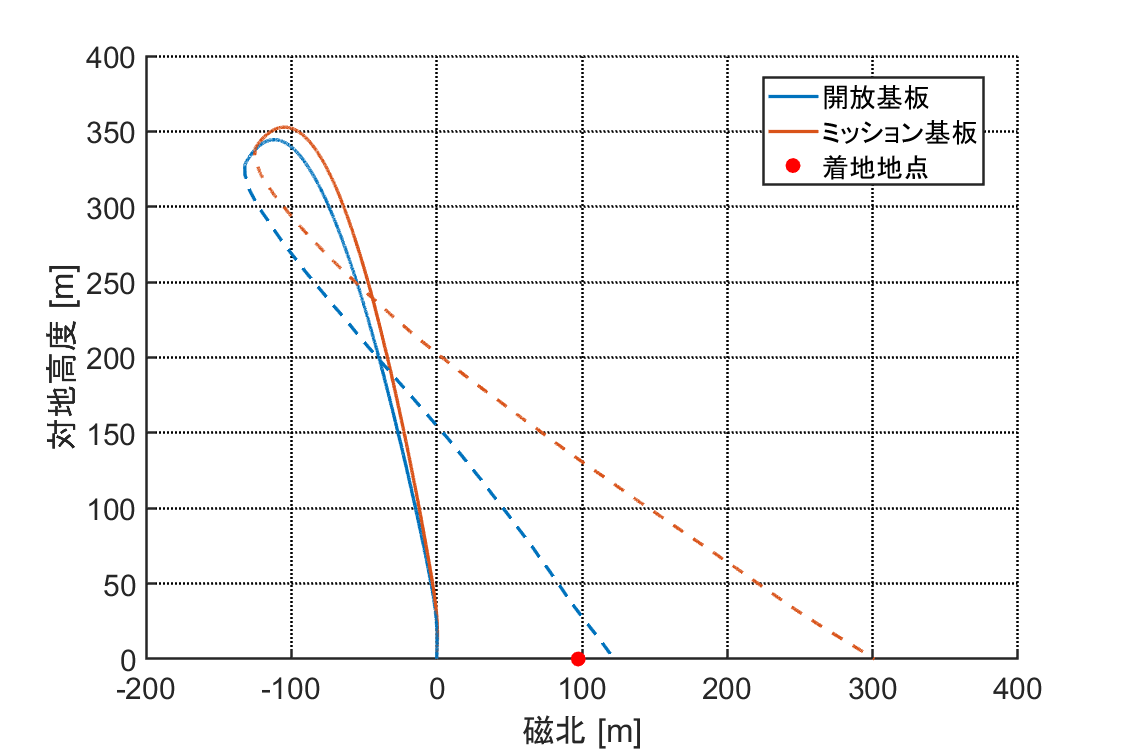
\includegraphics[width=75mm]{pic_sim/pos2_nh.png}
            \hspace{16mm} {\small[2]磁北-対地高度}
        \end{minipage}
    \end{tabular}
    \centering
    \begin{minipage}{.48\textwidth}
        \centering
        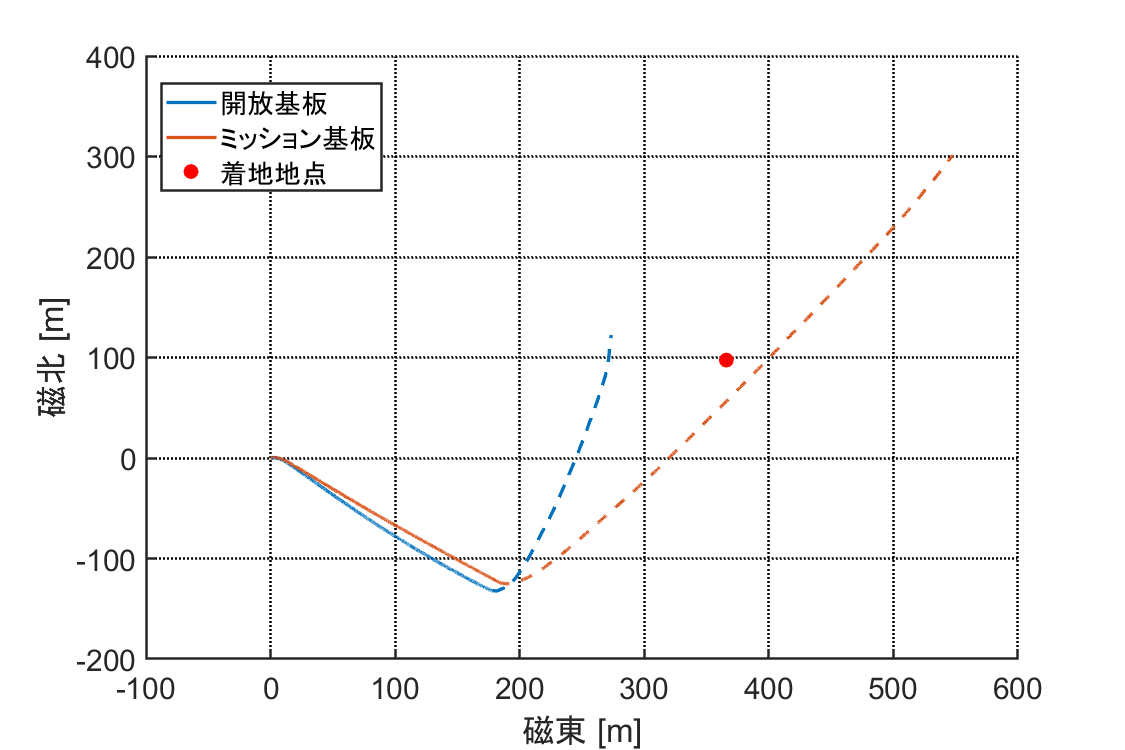
\includegraphics[width=75mm]{pic_sim/pos2_en.png}
        \hspace{16mm}{\small[3]磁東-磁北}
    \end{minipage}
    \caption{飛行経路}
    \label{fig:hikoukeiro}
\end{figure}

\begin{table}[H]
    \centering
    \caption{頂点座標}
    \label{tab:tyouten_kiban}
    \begin{tabular}{cccc}
        \hline
              & $x$ (\si{m}) & $y$ (\si{m}) & $z$ (\si{m}) \\\hline
        開放    & 146.2        & -111.8       & 344.5        \\
        ミッション & 155.1        & -104.7       & 352.8        \\
        \hline
    \end{tabular}
\end{table}

\begin{table}[H]
    \centering
    \caption{ランチクリア速度}
    \label{tab:launch_sokudo}
    \begin{tabular}{ccc}
        \hline
              & 時刻 (\si{s}) & ランチクリア速度 (\si{m/s}) \\
        \hline
        開放    & 0.42        & 23.19               \\
        ミッション & 0.42        & 22.69               \\
        \hline
    \end{tabular}
\end{table}

ここで、取得した加速度を地上座標系における機体の重心での値への変換は式を、各変数については表に示す。

\begin{equation}
    \bm{a}_e = C_{e/b}\left(\bm{a}_b-\bm{\omega}\times \bm{\omega}\times \bm{X}_s\right)-\bm{g}_e
    \label{eq:kasokudohennkann}
\end{equation}

\begin{table}[H]
    \centering
    \caption{式\eqref{eq:kasokudohennkann}諸元}
    \label{tab:}
    \begin{tabular}{lccr}
        \hline
        名称             & 変数            & 単位           & \multicolumn{1}{c}{値} \\
        \hline
        加速度ベクトル(取得値)   & $\bm{e}_b$    & \SI{}{m/s^2} & -                     \\
        加速度ベクトル(地上座標系) & $\bm{e}_e$    & \SI{}{m/s^2} & -                     \\
        角速度(機体座標系)     & $\bm{\omega}$ & \SI{}{rad/s} &                       \\
        座標変換行列         & $C_{e/b}$     & -            & -                     \\
        センサ位置(開放)      & $C_{e/b}$     & -            & -                     \\
        センサ位置(ミッション)   & $\bm{X}_s$    & $\SI{}{m}$   & -                     \\
        重力(地上座標系)      & $\bm{g}_e$    & \SI{}{m/s^2} & $(0,0,-9.8066)$       \\
        \hline
    \end{tabular}
\end{table}


図\ref{fig:taitisokudo}と図\ref{fig:hikoukeiro}からわかるように、2つのデータは頂点到達までは、対気速度及び飛行経路ともに大方一致していることがわかる。
頂点到達時の座標は表\ref{tab:tyouten_kiban}に示しているように、その差は\SI{14.0}{m}である。
独立した2つのセンサから同様の経路を算出できたことから、頂点到達前に関しては実際の対地速度及び飛行経路と近いものが得られたと考えられる。

一方で頂点到達以降に関しては、2つの算出結果に大きな差が生じていることがわかる。
これはパラシュート開傘時の運動がサンプリングレートより高い周波数の運動であることが原因と考えられる。
すなわち、6軸センサではパラシュート開傘後の運動を十分に追跡できなかったため、2つのセンサ間の差が拡大したと考えられる。

\subsubsection{高度}
\label{koudo}
離床時刻からの機体の高度は気圧センサのデータからも算出可能である。図\ref{fig:koudozikannkeika}に気圧センサ及び\ref{itisokudo}項で算出した高度の時間経過を、表にそれぞれの頂点到達時間及び最高到達高度を示す。

\begin{figure}[H]
    \centering
    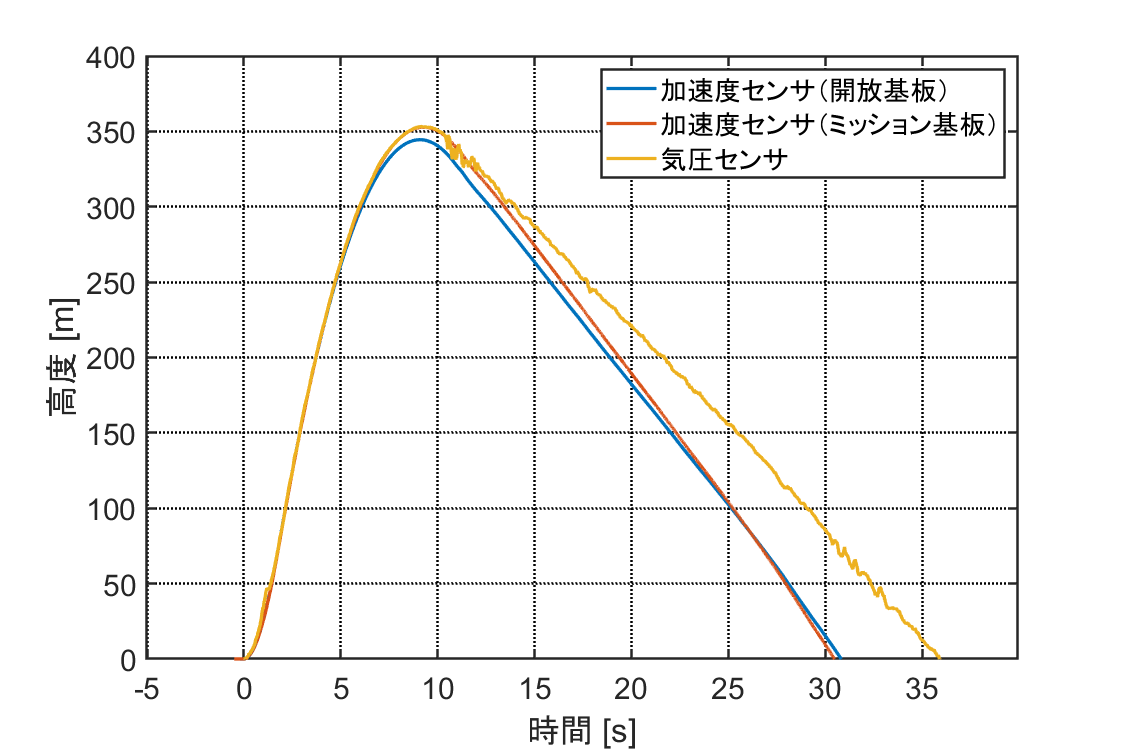
\includegraphics[width=0.7\linewidth]{pic_sim/pos_h.png}
    \caption{高度の時間経過}
    \label{fig:koudozikannkeika}
\end{figure}

\begin{table}[H]
    \centering
    \caption{頂点到達時間及び最高到達高度}
    \label{tab:tyouten}
    \begin{tabular}{ccc}
        \hline
              & 頂点到達時間 (\si{s}) & 高度 (\si{m}) \\\hline
        開放    & 9.08            & 344.5       \\
        ミッション & 9.27            & 352.8       \\
        気圧センサ & 9.48            & 353.0       \\
        \hline
    \end{tabular}
\end{table}

\begin{figure}[H]
    \centering
    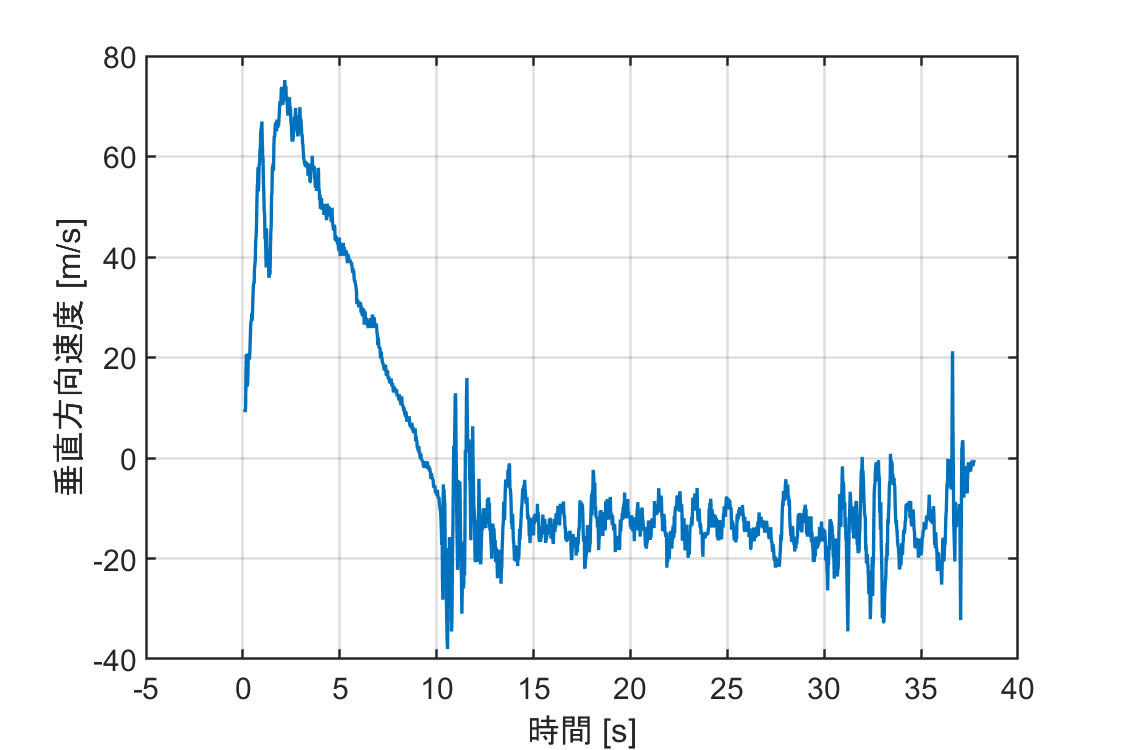
\includegraphics[width=0.7\linewidth]{pic_sim/hight_d.png}
    \caption{気圧センサから算出した垂直方向速度}
    \label{fig:suityoku_kiatu}
\end{figure}

図\ref{fig:suityoku_kiatu}は気圧センサから取得した高度を微分したものである。
ただし、変化を明瞭にするため0.4秒間、データ数にして20個のデータで移動平均を出したものをプロットしている。
パラシュート開傘時刻が離床から10.2秒後であり、比較的降下速度が安定しているのが\SI{12.5}{s}付近であることから、
開傘から終端速度到達までに\SI{2.5}{s}ほどかかっていることがうかがえる。
終端速度に関しては、\SI{15.0}{s}から\SI{30.0}{s}の間に\SI{274.3}{m}降下していることから、終端速度は\SI{13.2}{m/s}であることがわかった。
表\ref{tab:kouryoku_shogen}に記載する諸元を用いて計算した結果、パラシュートの抗力係数は1.27であることがわかった。

\begin{table}[H]
    \centering
    \caption{抗力係数算出諸元}
    \label{tab:kouryoku_shogen}
    \begin{tabular}{lcr}
        \toprule
        \multicolumn{1}{c}{諸元名} & 単位          & \multicolumn{1}{c}{値} \\
        \midrule
        降下速度                    & \si{m/s}    & 13.71                 \\
        燃焼終了後重量                 & \si{kg}     & 5.894                 \\
        気体密度                    & \si{kg/m^3} & 1.144                 \\
        代表面積                    & \si{m^3}    & 0.422                 \\
        \midrule
        抗力係数                    & -           & 1.27                  \\
        \bottomrule
    \end{tabular}
\end{table}

\subsubsection{姿勢}
取得した角速度データから、飛行中の機体の姿勢を表すクォータニオンを算出した。図\ref{fig:quatarnionhikaku}にそれぞれの基板のから算出した値を示す。
またこれらクォータニオンを動翼の制御に使用したyxzオイラー角に変更したものを図\ref{fig:oirahikaku}に示す。

\begin{figure}[H]
    \centering
    \begin{minipage}{.85\textwidth}
        \centering
        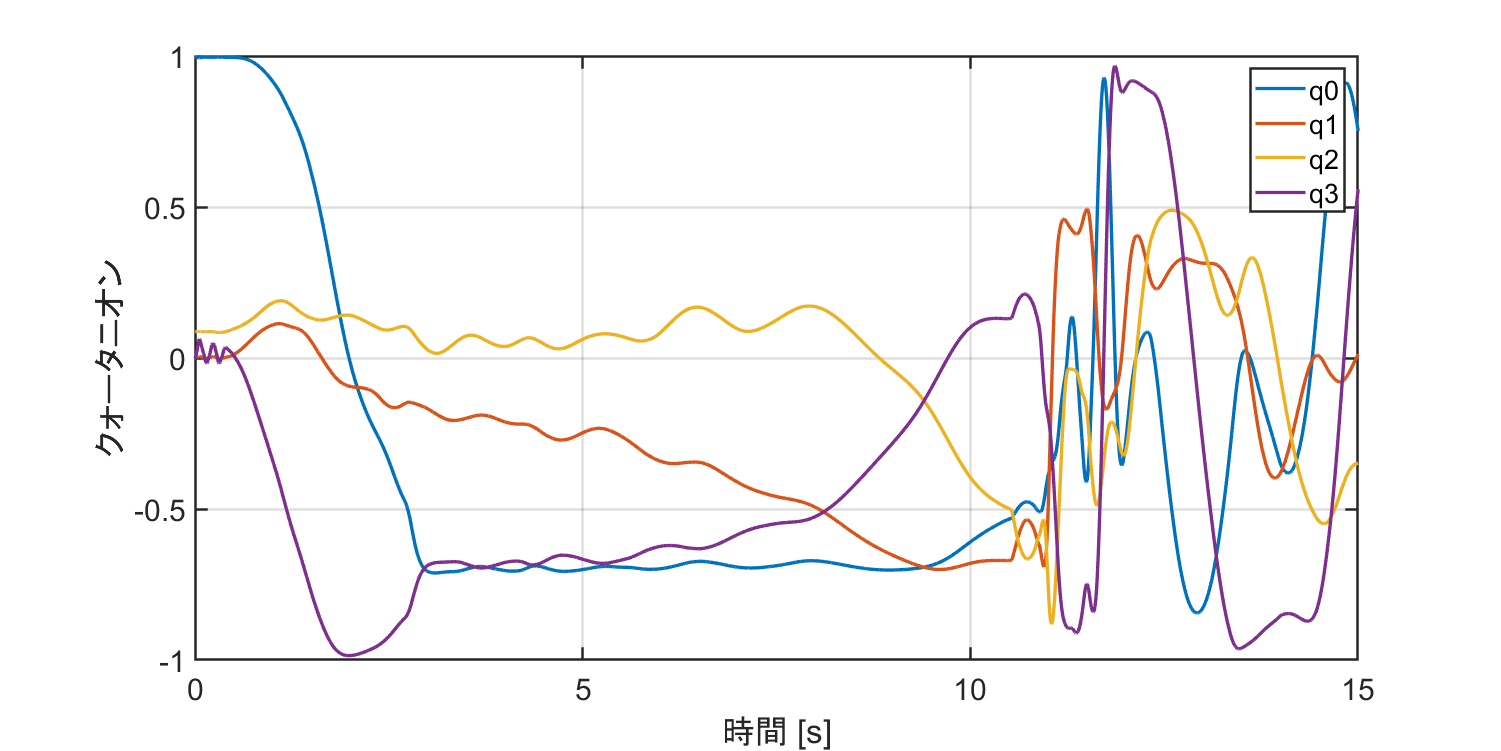
\includegraphics[width=0.95\linewidth]{pic_sim/qua_no_s.png}
        \hspace{16mm}{\small[1]開放基板}

        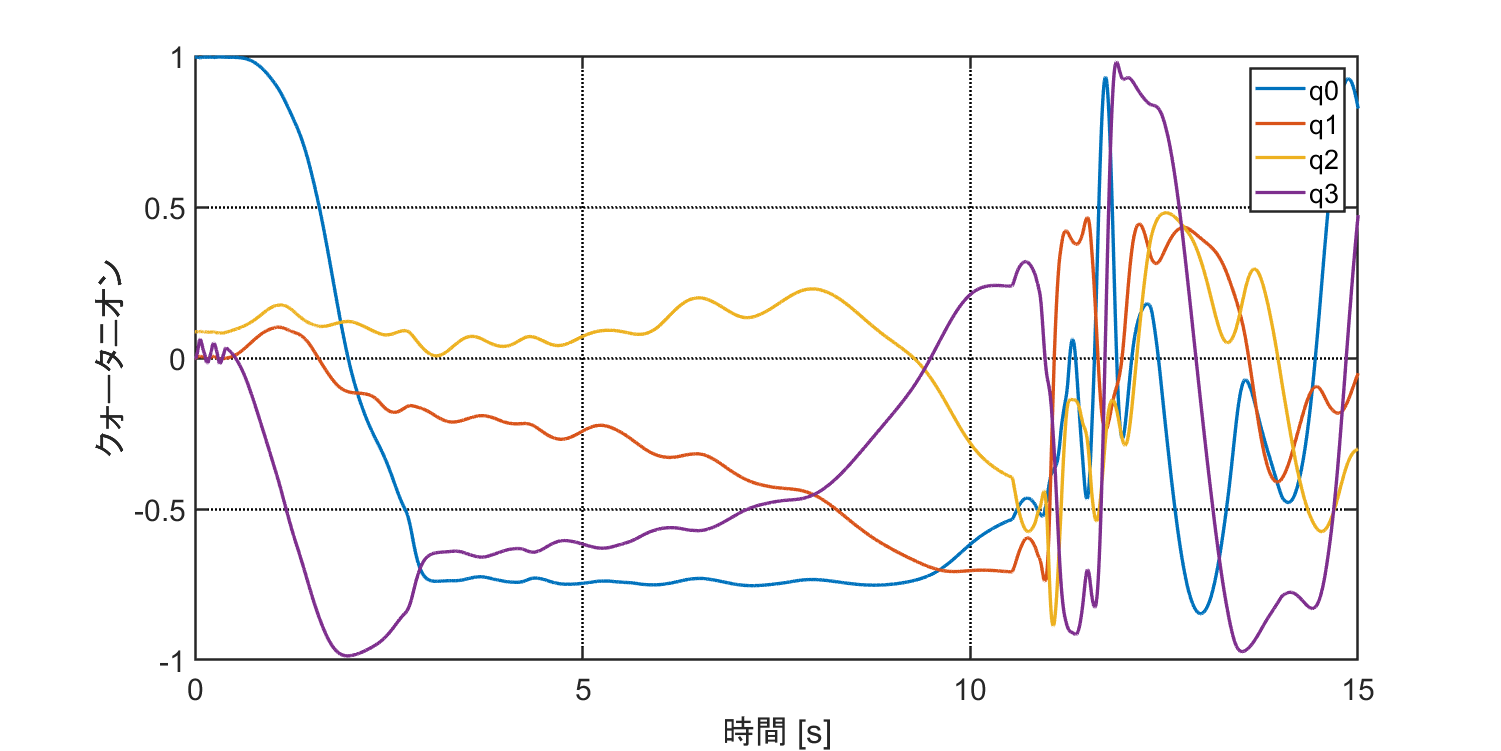
\includegraphics[width=0.95\linewidth]{pic_sim/qua_ta_s.png}
        \hspace{16mm}{\small[2]ミッション基板}
    \end{minipage}
    \caption{算出したクォータニオン}
    \label{fig:quatarnionhikaku}
\end{figure}

\begin{figure}[H]
    \centering
    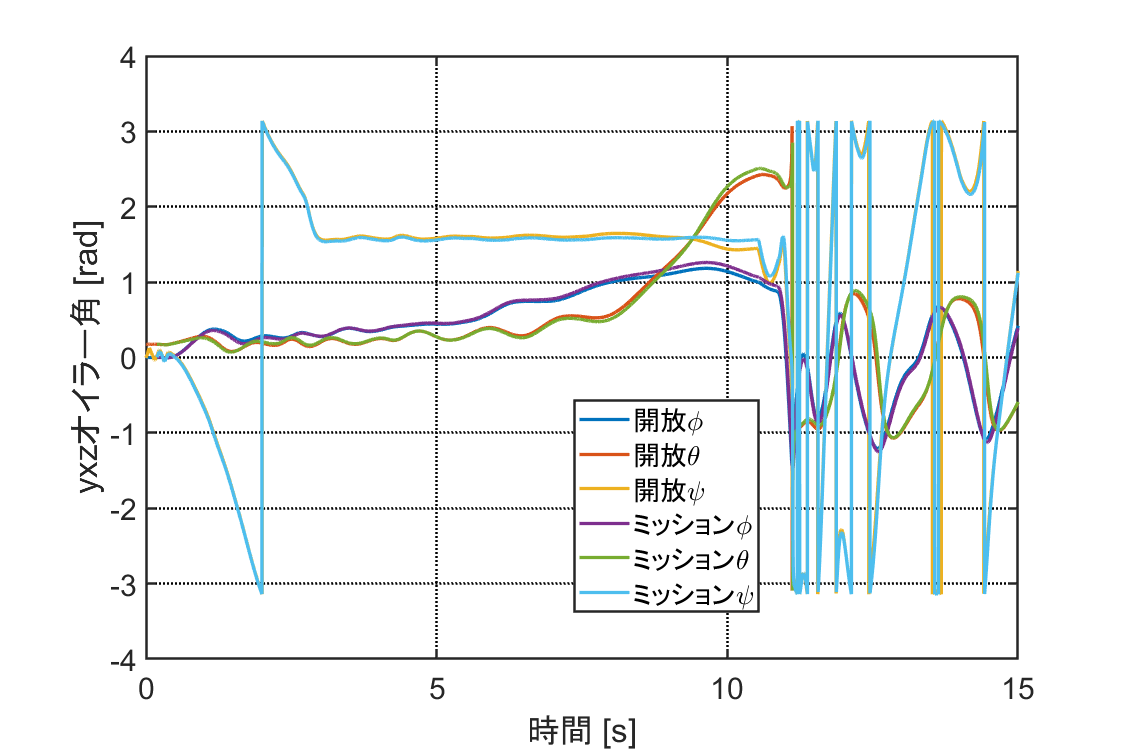
\includegraphics[width=0.65\linewidth]{pic_sim/euler2.png}
    \caption{yxzオイラー角の比較}
    \label{fig:oirahikaku}
\end{figure}

\begin{figure}[H]
    \begin{tabular}{cc}
        \begin{minipage}{.48\textwidth}
            \centering
            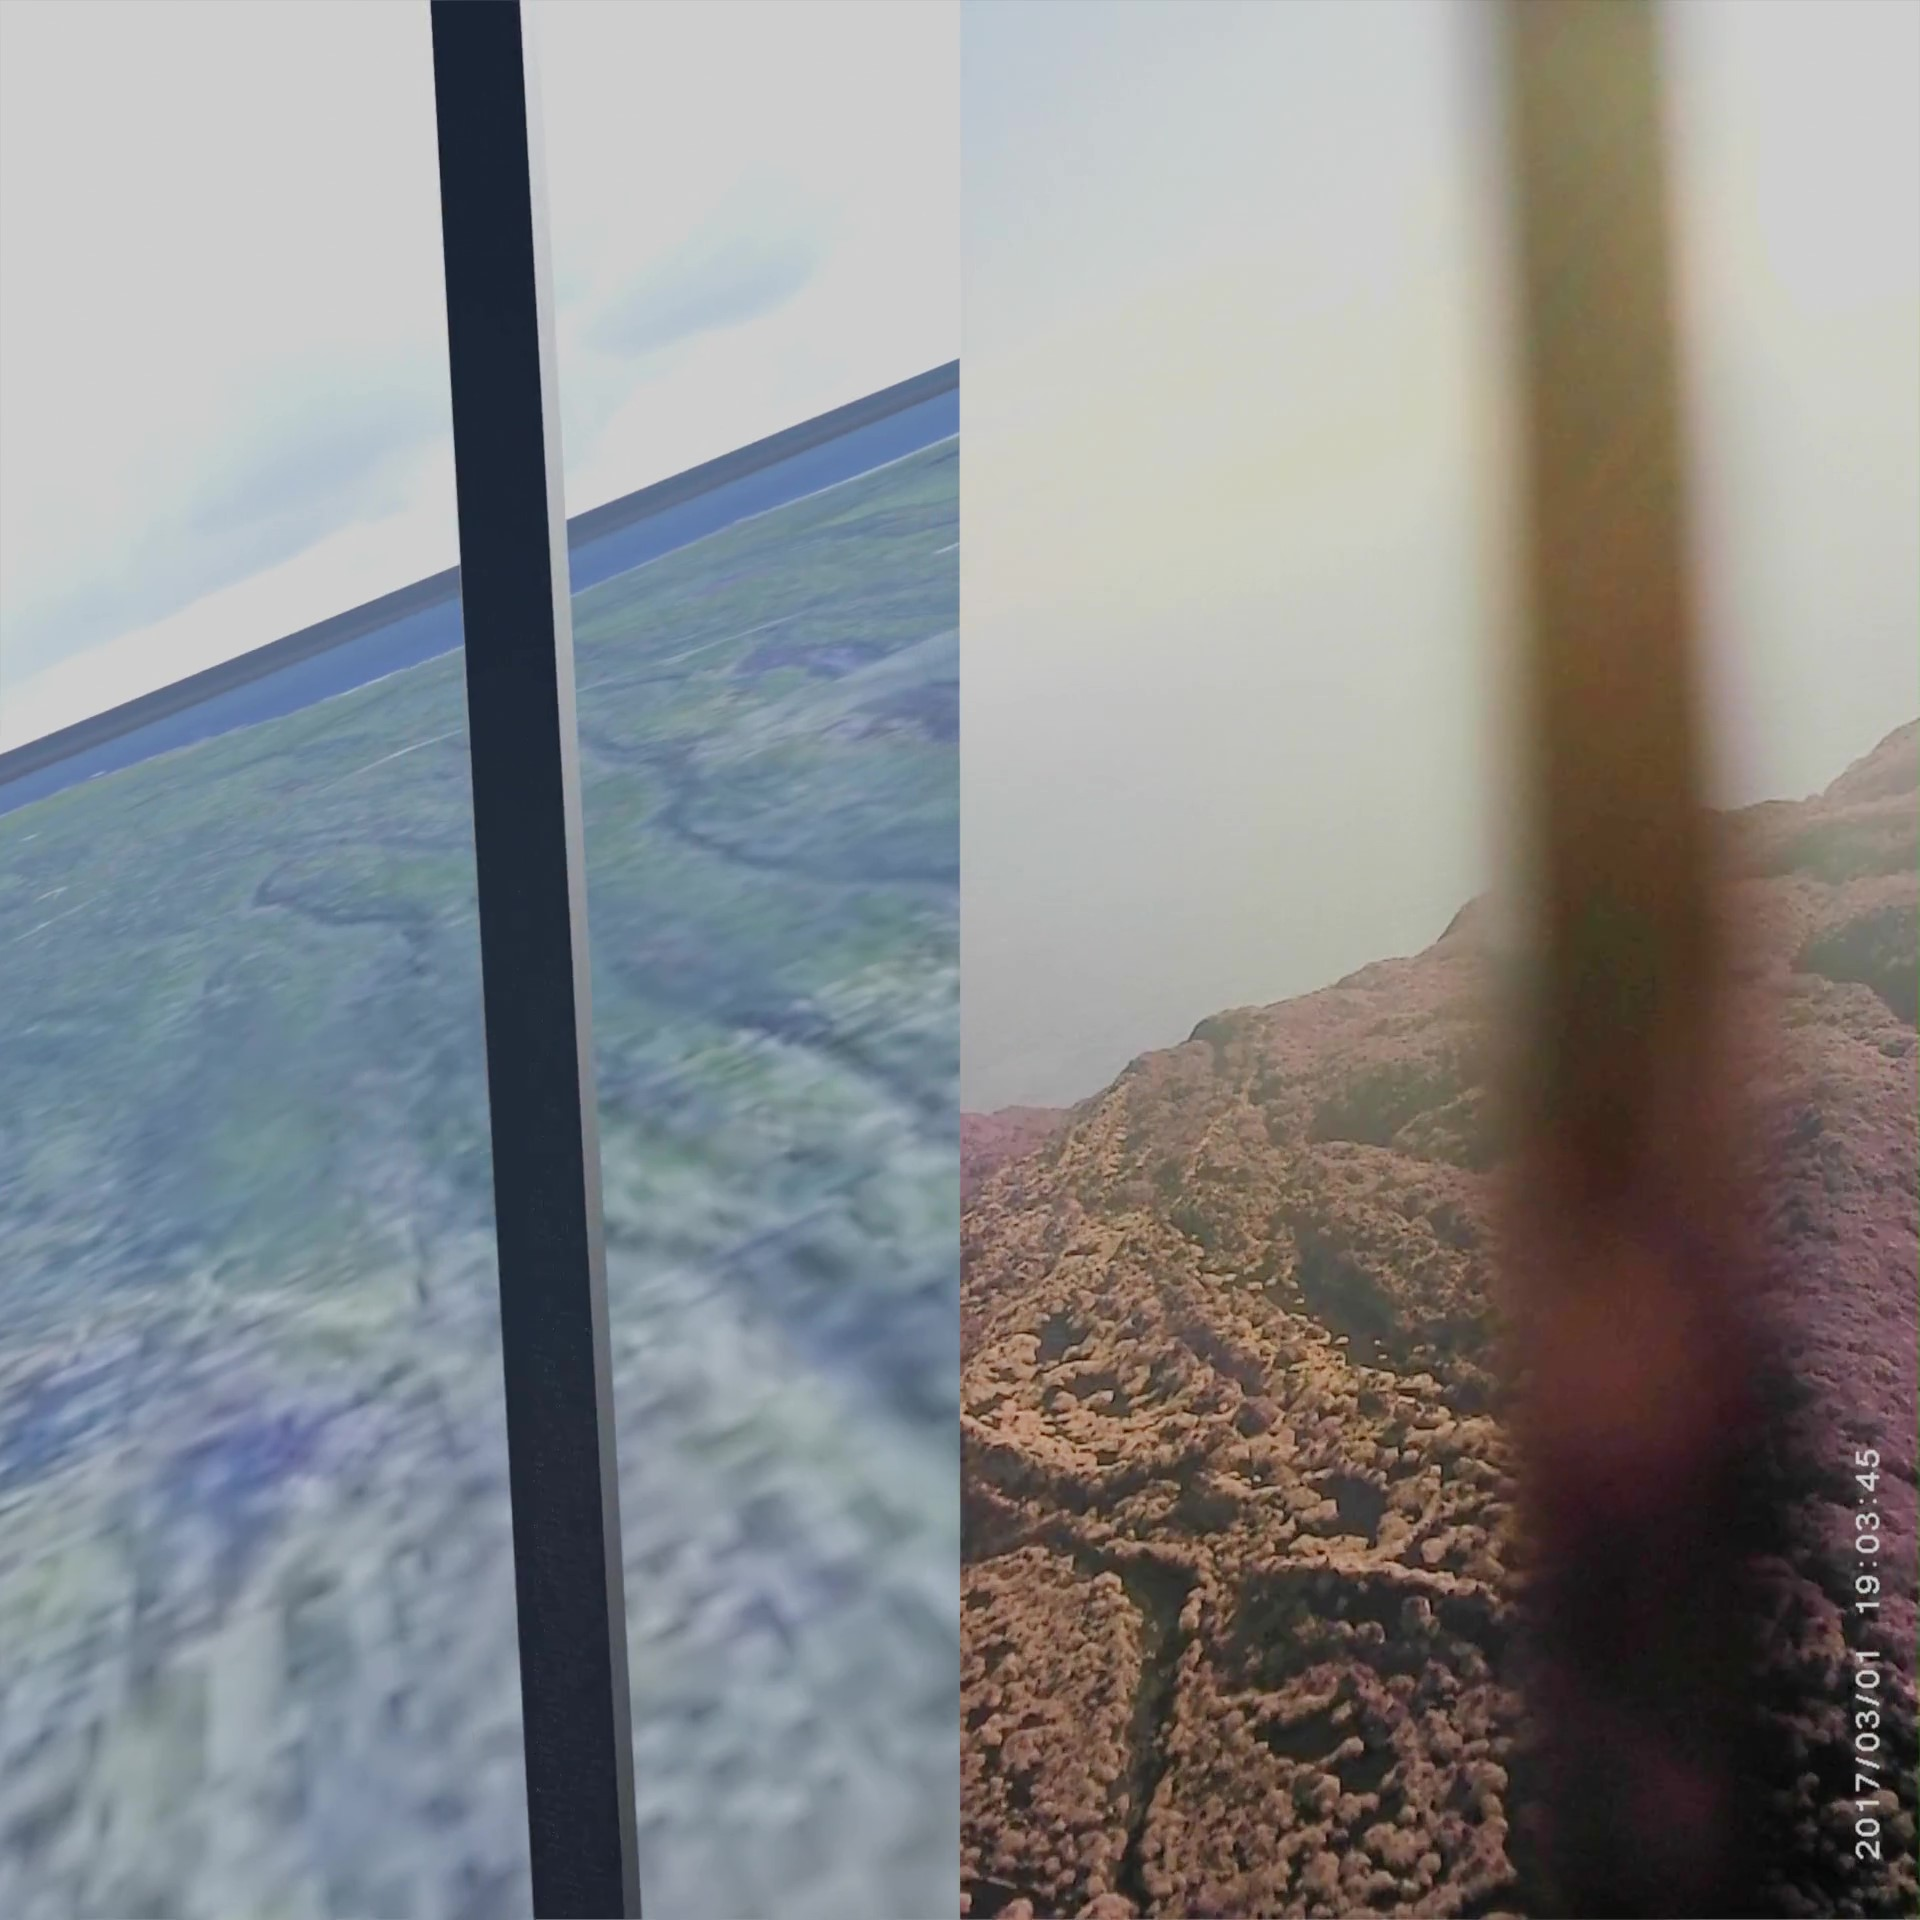
\includegraphics[width=75mm]{pic_sim/compare_5.jpg}
            \hspace{16mm} {\small[1] 離床5秒後(左:CG、右:機体カメラ)}
        \end{minipage}
        \begin{minipage}{.48\textwidth}
            \centering
            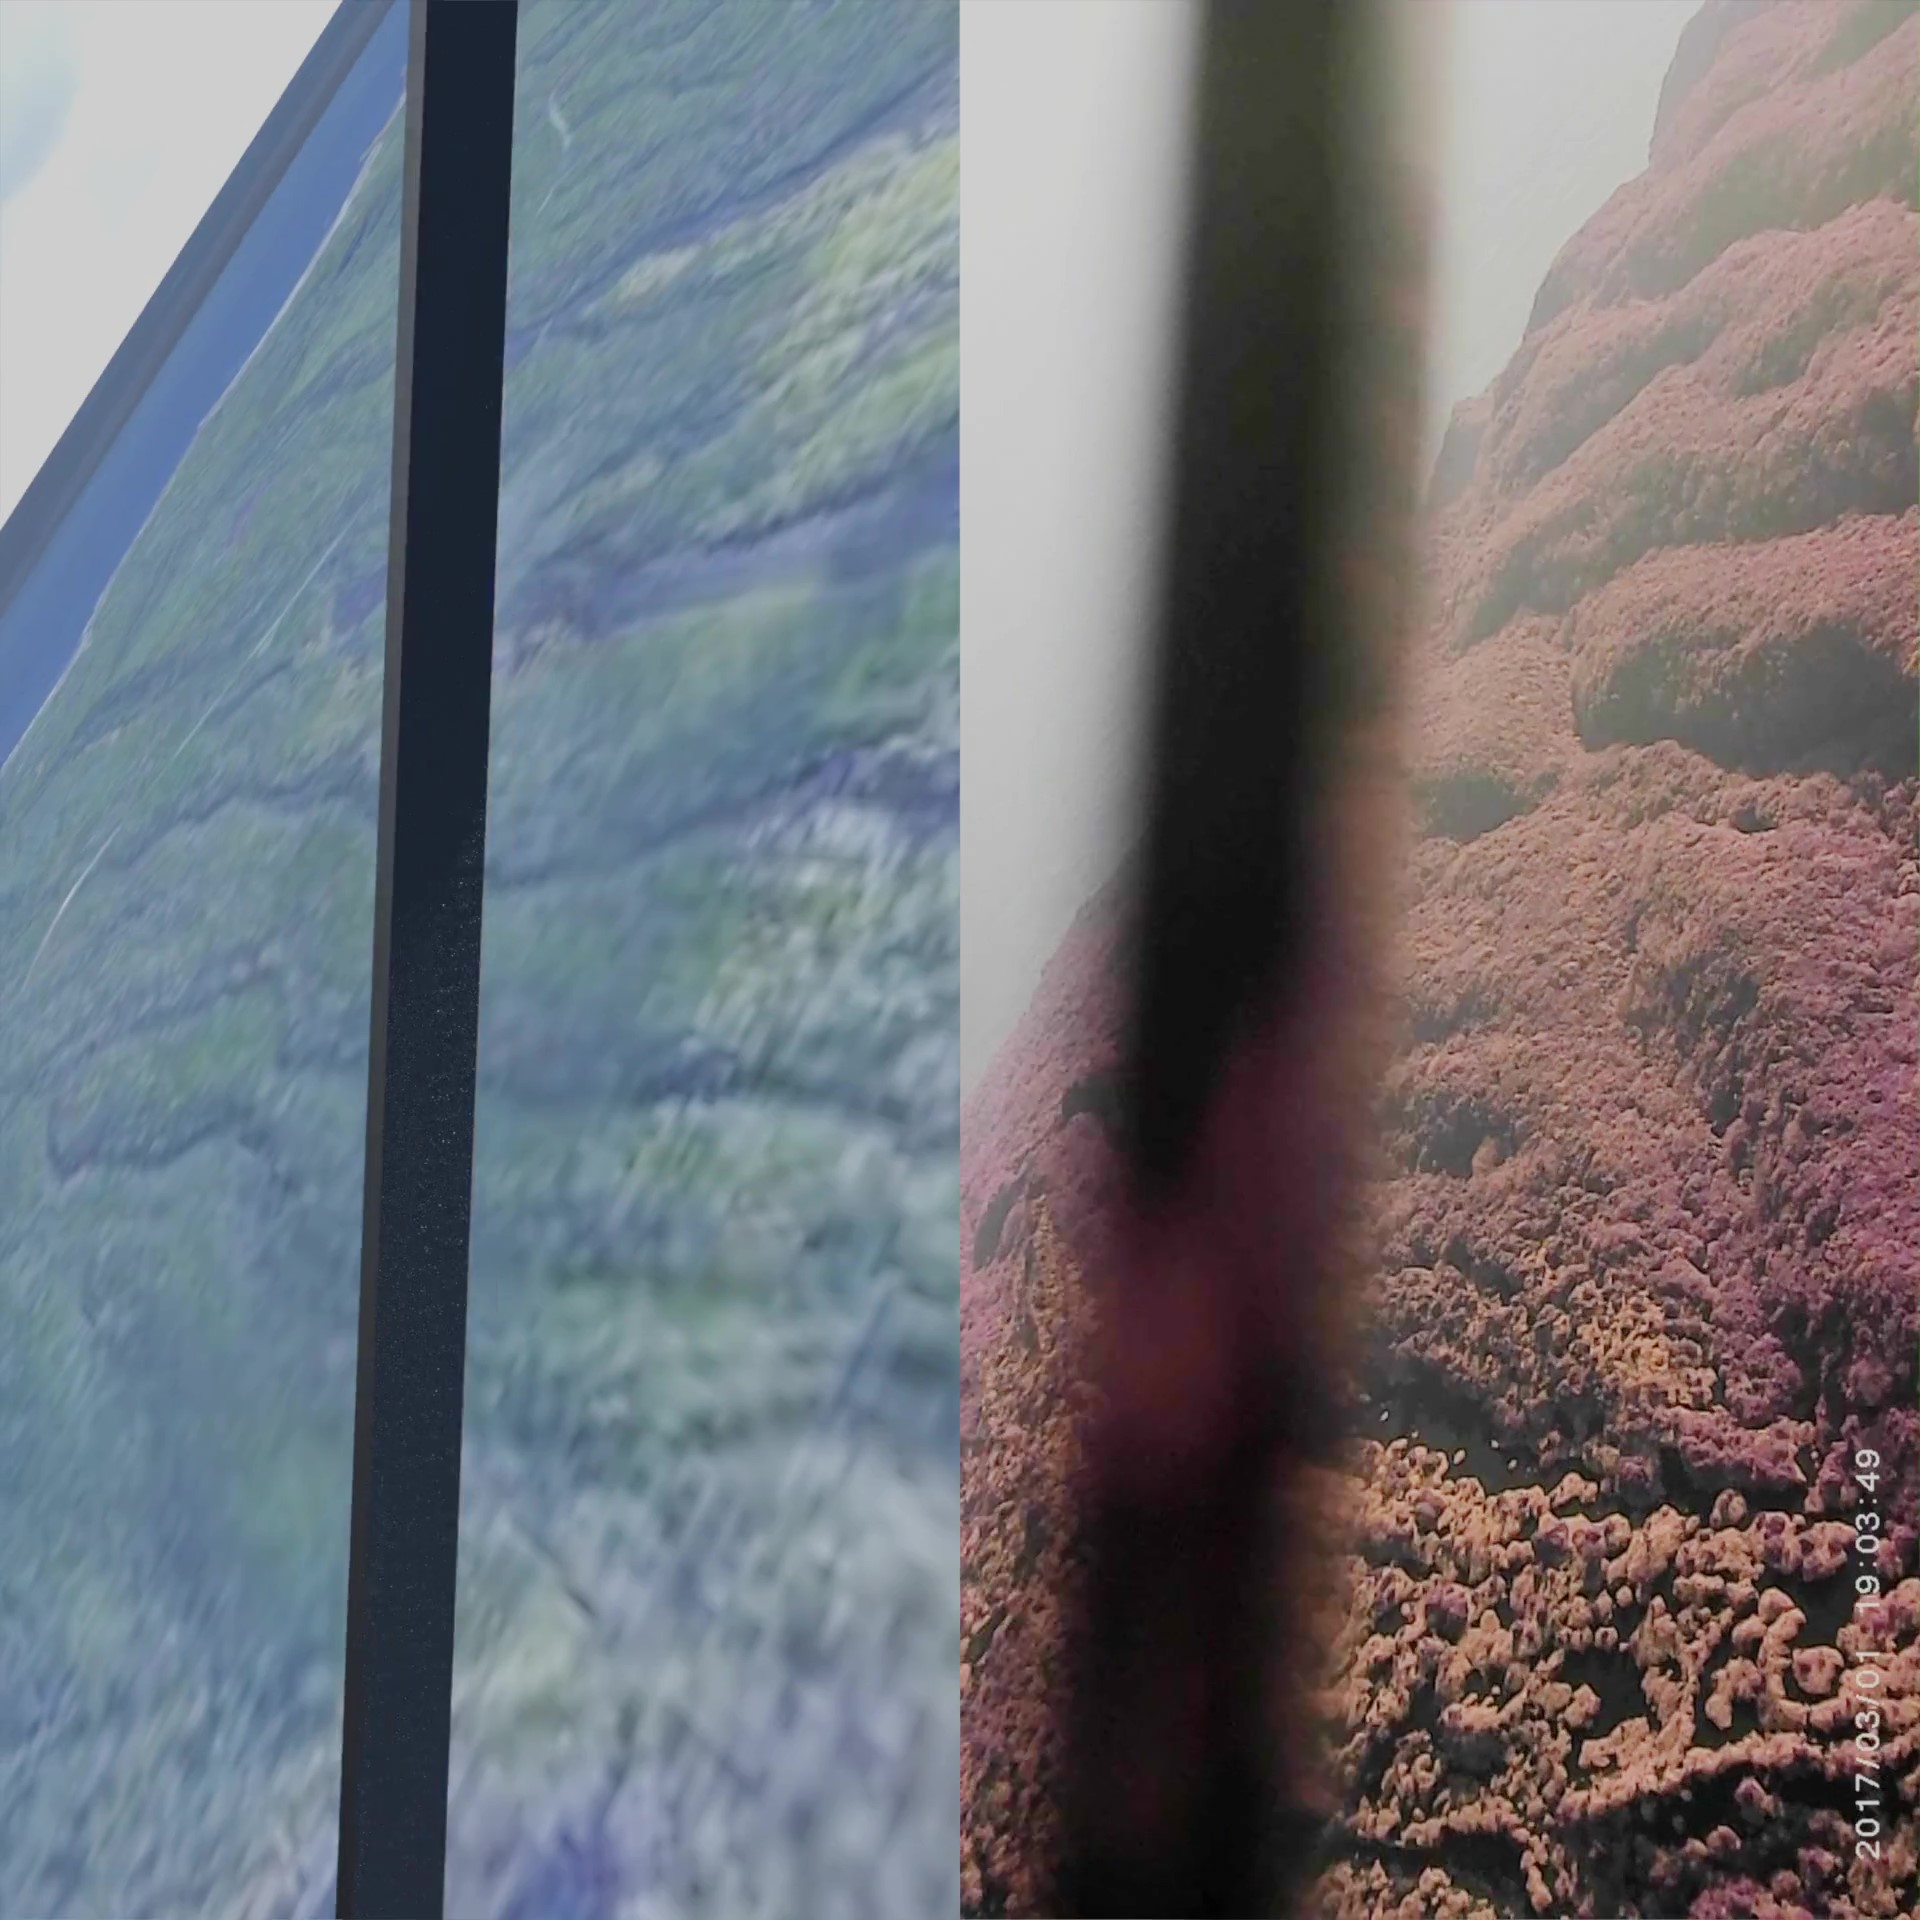
\includegraphics[width=75mm]{pic_sim/compare_8.jpg}
            \hspace{16mm} {\small[2] 離床8秒後(左:CG、右:機体カメラ)}
        \end{minipage}
    \end{tabular}
    \centering
    \caption{CGと機体カメラの映像の比較}
    \label{fig:dougahikaku}
\end{figure}

図\ref{fig:oirahikaku}に示した通り、それぞれの基板のセンサから算出した姿勢にほとんど差異は見られなかった。パラシュート開傘以前において、その差の最大値は$\psi$で\SI{6.9}{deg}であった。
図\ref{fig:dougahikaku}に示しているように、機体に搭載したカメラからの動画映像と、算出したクォーターニオンの値を用いて作成したCG映像を比較しても、その差がほとんど見られないことが確認できた。

次に、取得した磁気センサの値の精度を評価する。
磁気センサの零点補正を行うため、最小二乗法を用いて球面フィッテングを行った。補正した結果を図\ref{fig:tiziki}に、ノルムの時間変化を図\ref{fig:tizikinorumu}に示す。


\begin{figure}[H]
    \centering
    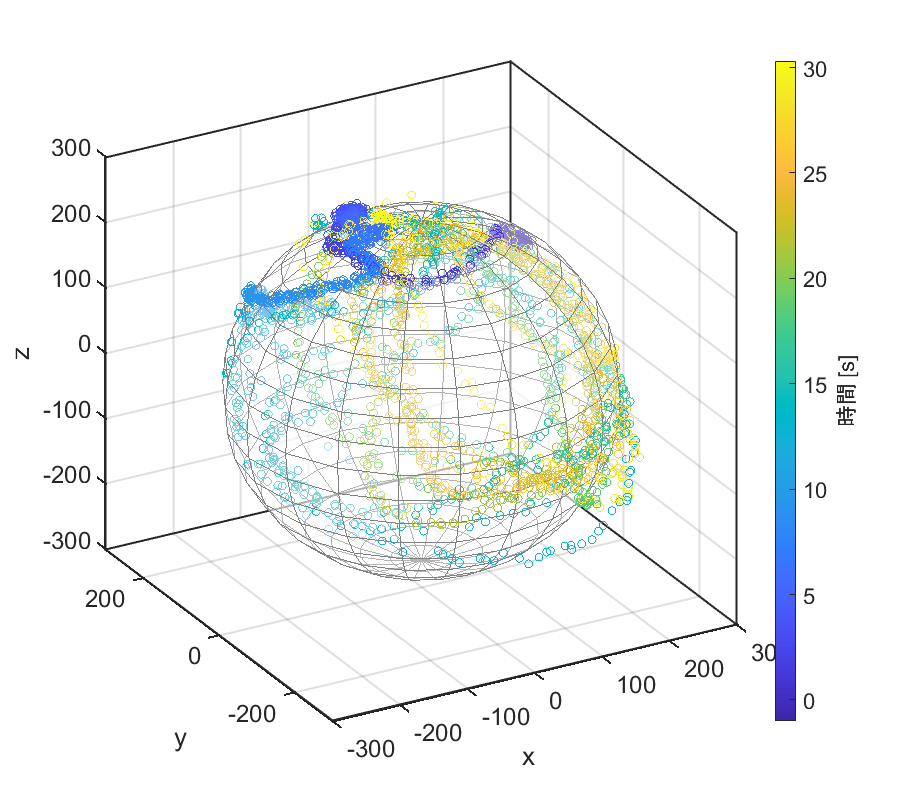
\includegraphics[width=0.7\linewidth]{pic_sim/mag_fix.png}
    \caption{零点補正後の磁気センサ}
    \label{fig:tiziki}
\end{figure}
\begin{figure}[H]
    \centering
    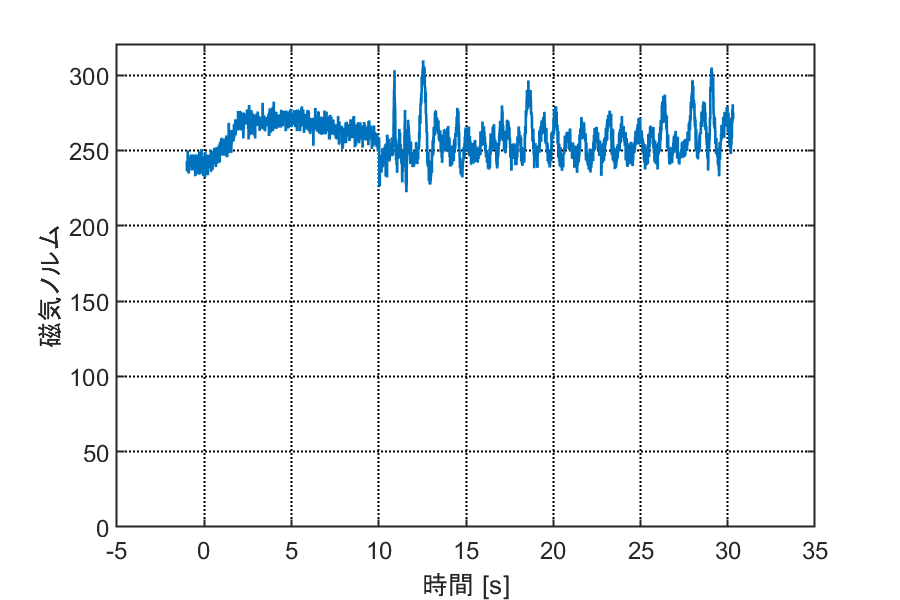
\includegraphics[width=0.7\linewidth]{pic_sim/mag_norm.png}
    \caption{零点補正後の磁気センサノルム}
    \label{fig:tizikinorumu}
\end{figure}

ここで算出したクォーターニオンを用いて磁気センサの値を地上座標系に変換したものを図\ref{fig:tizikihennkann}に示す。

\begin{figure}[H]
    \centering
    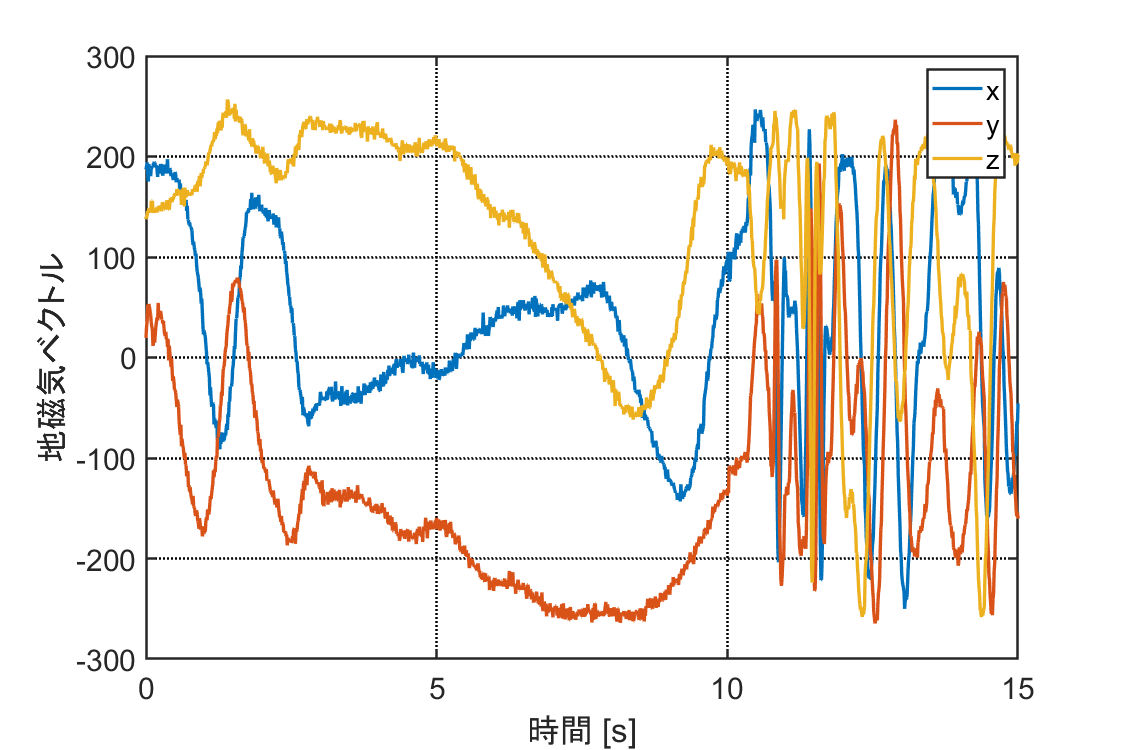
\includegraphics[width=0.7\linewidth]{pic_sim/mag_rot.png}
    \caption{磁気ベクトルの各成分(地上座標系)}
    \label{fig:tizikihennkann}
\end{figure}

本来は地磁気ベクトルが定ベクトルであるため、図\ref{fig:tizikihennkann}に示した各軸の値は一定になるはずである。
算出したクォーターニオンは精度が確認されていることから、磁気センサの値に何らかの問題があることがわかる。
ノルムの時間変化が小さくベクトルも球面上に存在しており、理想的なデータであったのにも関わらずこのような結果となった原因は現状不明である。


\subsubsection{推力履歴}
\label{suiryokurireki}
加速度データから打ち上げ時のエンジンの推力履歴を算出した。開放基板、ミッション基板から算出したものと、直近の2022年7月に実施された燃焼試験での値を図\ref{fig:suiryokurireki}に示す。
また推力に関する各諸元を表\ref{tab:nenshoushogen}に、加速度データから推力の算出式を式\eqref{eq:T}に、各変数を表\ref{tab:eqshogen}に示す。

\begin{figure}[H]
    \centering
    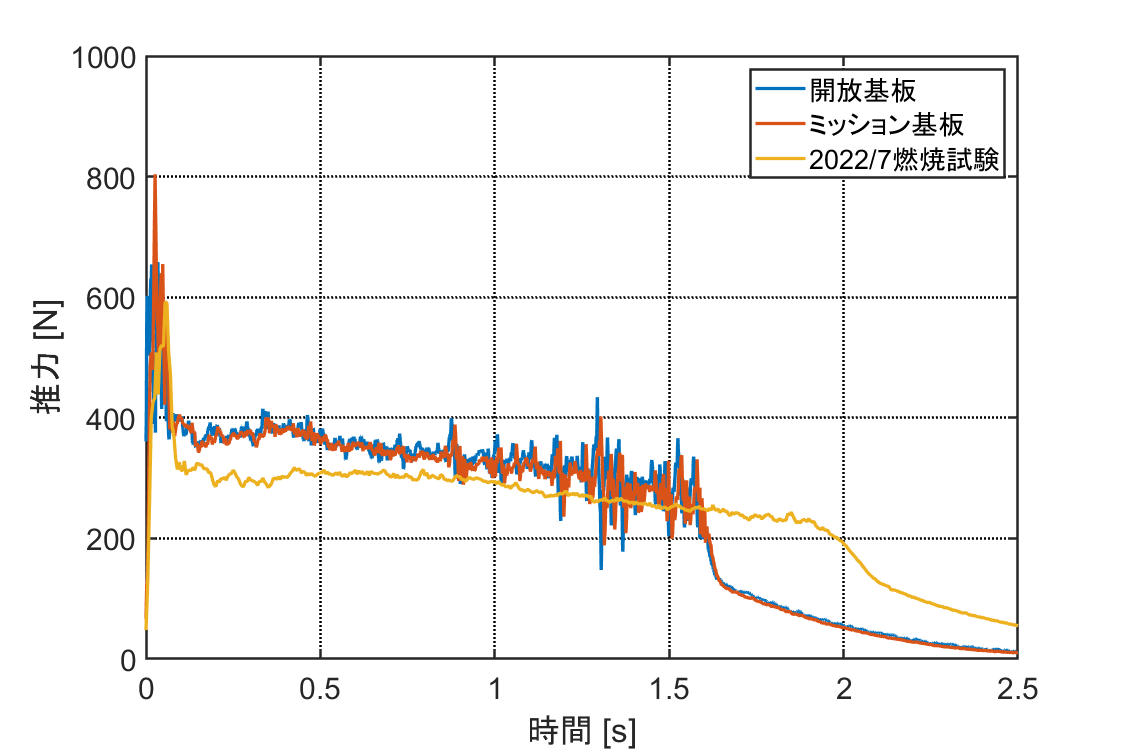
\includegraphics[width=0.7\linewidth]{pic_sim/acc_thrust.png}
    \caption{推力履歴の比較}
    \label{fig:suiryokurireki}
\end{figure}



\begin{table}[H]
    \centering
    \caption{燃焼諸元}
    \label{tab:nenshoushogen}
    \begin{tabular}{lcrrr}
        \hline
        名称        & 単位         & \multicolumn{1}{c}{開放} & \multicolumn{1}{c}{ミッション} & \multicolumn{1}{c}{7月燃焼試験} \\
        \hline
        トータルインパルス & \SI{}{N.s} & 596                    & 581                       & 628                        \\
        平均推力      & \SI{}{N}   & 273                    & 280                       & 226                        \\
        比推力       & \SI{}{s}   & 169                    & 165                       & 174                        \\
        作動時間      & \SI{}{s}   & 2.18                   & 2.08                      & 2.79                       \\
        \hline
    \end{tabular}
\end{table}

\begin{equation}
    T = a_z\qty(M_0 + \frac{M_1-M_0}{b_t}t)+\frac{1}{2}C_d \rho S V^2
    \label{eq:T}
\end{equation}

\begin{table}[H]
    \centering
    \caption{式\eqref{eq:T}諸元}
    \label{tab:eqshogen}
    \begin{tabular}{lccr}
        \toprule
        名称         & 変数       & 単位         \\
        \midrule
        推力         & $T$      & \si{N}     \\
        z軸加速度(センサ) & $a_{sz}$ & \si{m/s^2} \\
        燃焼前質量      & $M_0$    & \si{kg}    \\
        燃焼後質量      & $M_1$    & \si{kg}    \\
        作動時間       & $b_t$    & \si{s}     \\
        時刻         & $t$      & \si{s}     \\
        \bottomrule
    \end{tabular}
\end{table}

図\ref{fig:suiryokurireki}の青線は打上実験時の開放基板から算出した推力を、赤線はミッション基板から算出した推力を、また黄線は2022年7月の燃焼実験時の推力をそれぞれ表している。

燃焼実験時と打ち上げ実験時の推力履歴を比較すると、打ち上げ実験時の方が作動時間が短く、またそれに伴ってトータルインパルスも小さくなっている。
この原因としては,燃焼実験と打ち上げ実験で供給されている酸化剤の量が異なることが考えられる。燃焼実験では、タンク圧の計測を行っており、圧力センサ取り付け用の流路が存在している。
打ち上げ実験時には、このような流路は存在しないため、この流路の分の酸化剤が供給されておらず、これが作動時間やトータルインパルスに影響を与えたと考えられる。

\begin{comment}
\subsubsection{ロール運動関連}

ロール運動について取得した角速度データから、ロール運動関連の空力係数である定常ロールモーメント係数$C_{l0}$、ロール減衰モーメント係数$C_{l_p}$、動翼ロールモーメント係数$C_{l_{\delta_a}}$を推定する。
式?にロール方向の回転運動方程式を示す。また、離床から5秒間のロール角加速度、ロール角速度、対地速度、動翼舵角を図?に示す。
\textcolor{red}{$\omega_a$じゃなくて$p$のほうがいいんかな}
\begin{align}
    \label{qe:ro-ruunndouhouteiisiki}
    \dot{\omega}_x & = L_p\omega_x+L_0+L_{\delta_a}\delta_a       \\
    L_P            & = \frac{\rho V^2Sb^2}{4I_{xx}}C_{l_p}        \\
    L_0            & = \frac{\rho V^2Sb}{2I_{xx}}C_{l_p}          \\
    L_P            & = \frac{\rho V^2Sb}{2I_{xx}}C_{l_{\delta_a}}
\end{align}

\begin{figure}[H]
    \begin{tabular}{cc}
        \begin{minipage}{.48\textwidth}
            \centering
            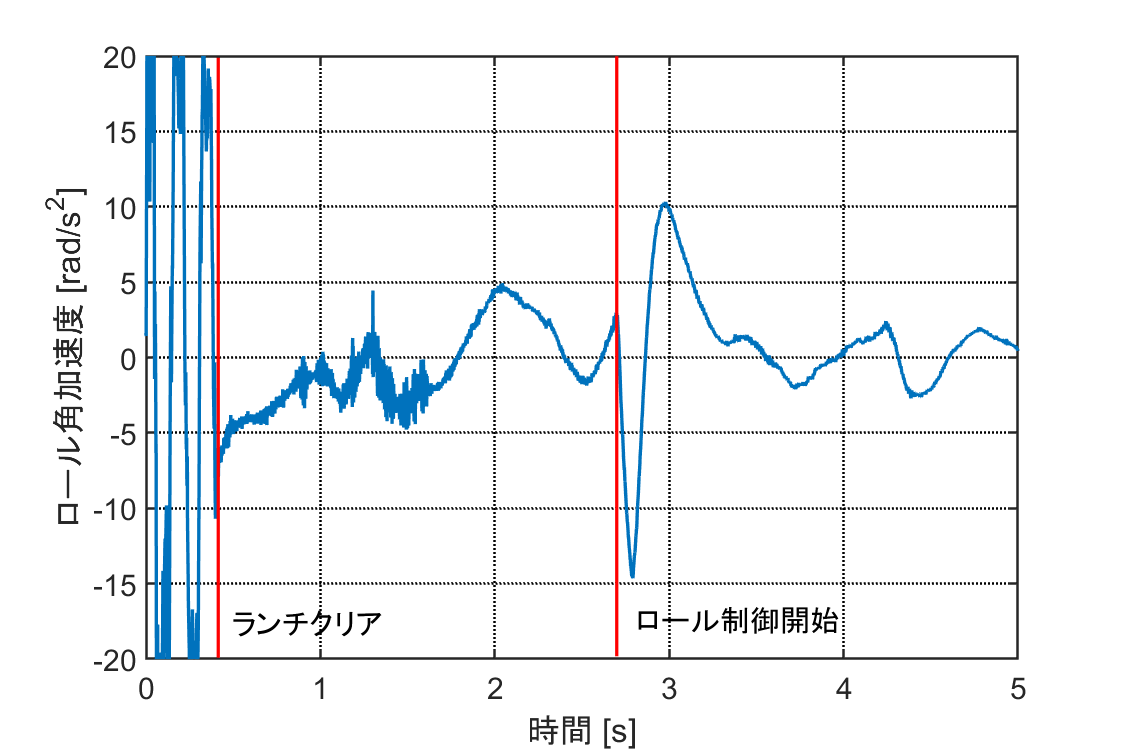
\includegraphics[width=75mm]{pic_sim/omega_dot.png}
            \hspace{16mm} {\small[1]ロール角加速度}
        \end{minipage}
        \begin{minipage}{.48\textwidth}
            \centering
            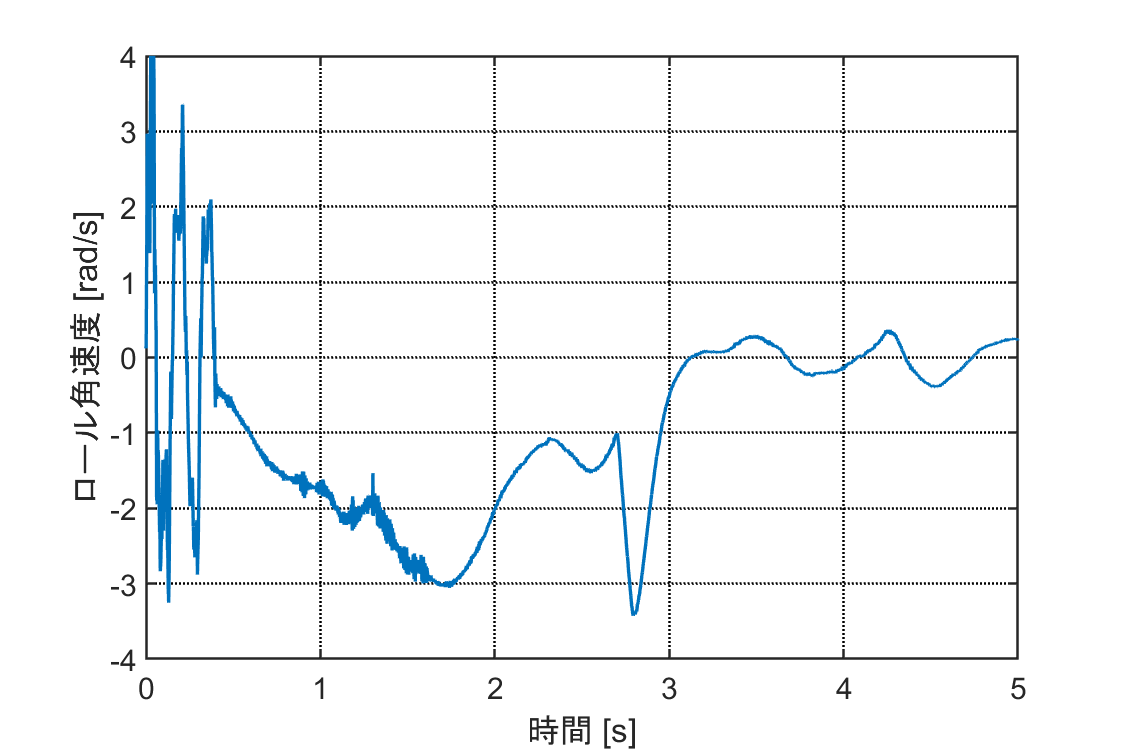
\includegraphics[width=75mm]{pic_sim/omega_x.png}
            \hspace{16mm} {\small[2]ロール角速度}
        \end{minipage}
    \end{tabular}
    \begin{tabular}{cc}
        \begin{minipage}{.48\textwidth}
            \centering
            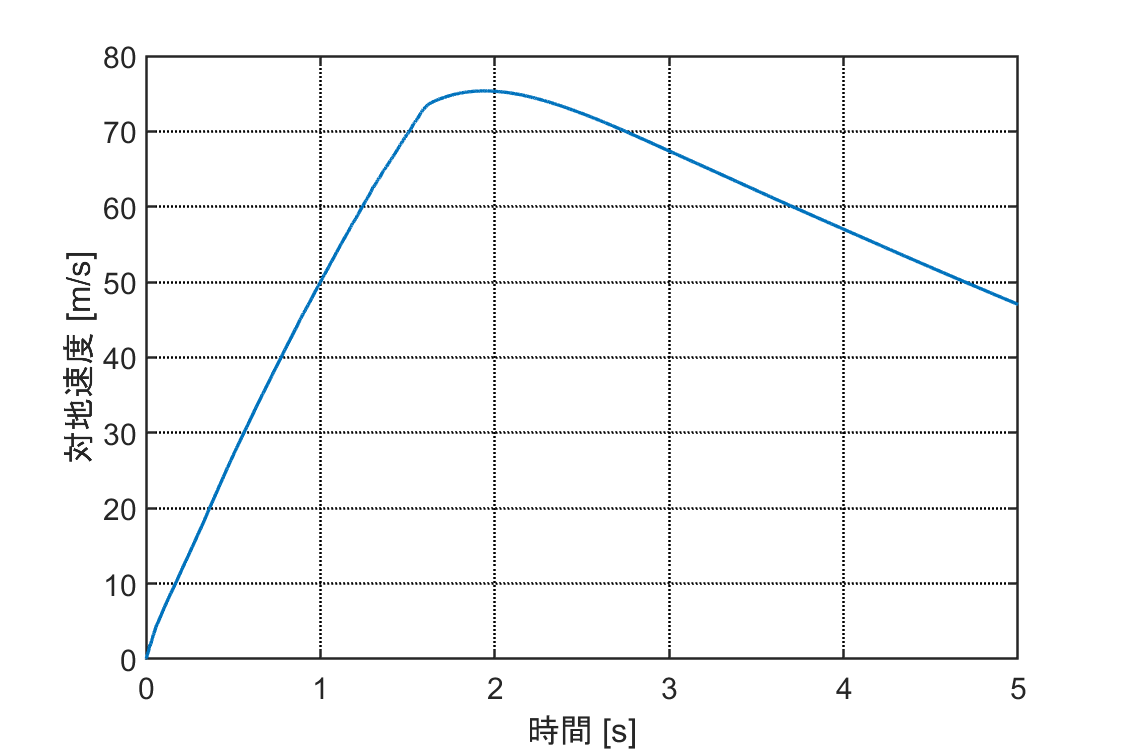
\includegraphics[width=75mm]{pic_sim/Ven.png}
            \hspace{16mm} {\small[3]対地速度}
        \end{minipage}
        \begin{minipage}{.48\textwidth}
            \centering
            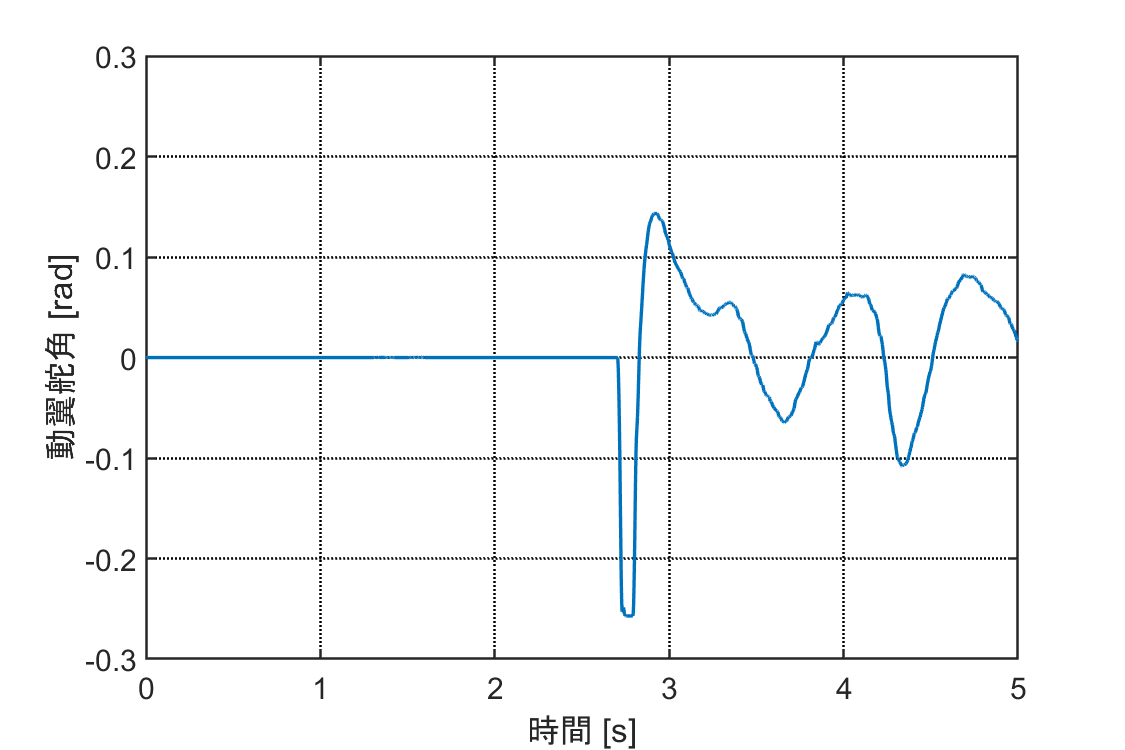
\includegraphics[width=75mm]{pic_sim/delta_a.png}
            \hspace{16mm} {\small[4]動翼舵角}
        \end{minipage}
    \end{tabular}
    \caption{ロール運動関連飛行データ}
    \label{fig:rollkannrenn}
\end{figure}

ここで、機軸周り角加速度$\dot{\omega}_x$の時間推移は、式\eqref{qe:ro-ruunndouhouteiisiki}において対気速度$V$、角速度$\omega_x$、動翼舵角$\delta_a$のみを変数と考え、慣性モーメントの時間変化を無視すると
\begin{equation}
    \label{eq:omegamoderu}
    \dot{\omega}_x = a_0 V^2+ a_1 V^2 \omega_x + a_2V^2\delta_a
\end{equation}
とモデル化できる。ただし$a_0,a_1,a_2$はそれぞれの空力係数をに関する定数である。また、角速度については角速度センサ、動翼舵角に関してはエンコーダーのログデータ、対気速度は\ref{itisokudo}項で算出した対地速度を対気速度として使用しする\footnote{シミュレーションの結果、風速\SI{3}{m/s}の条件下における対気速度と対地速度の差は離床から?sまでは?%以下であり、十分対地速度を対気速度として使用可能である。\textcolor{red}{まだやってない}}。
目的の空力係数を算出するためには式?が図?に示すような時間変化となる$a_0,a_1$を算出できればよい。そこで最小二乗法を用いて算出する。

まず、ランチクリア後から制御直前(?\SI{}{s}~?\SI{}{s})に注目して空力係数を算出する。この間、動翼の舵角は常に\SI{0}{deg}であるため式\eqref{eq:omegamoderu}の右辺第3項を無視し、$a_0,a_1$の2つを求める。
\end{comment}


\subsection{事後シミュレーション}
打ち上げ実験後に、打ち上げ10分前に計測した風向風速データをもとにべき法則を用いて事後シミュレーションを行った。
風向風速データを表\ref{tab:huukouhuusoku}に、べき法則の各パラメーターを表\ref{tab:bekihousoku}に示す。

\begin{table}[H]
    \begin{minipage}[t]{0.55\hsize}
        \centering
        \caption{風向風速}
        \begin{tabular}[t]{lc} \hline
            風向 & 磁南(\SI{0}{deg}) \\
            風速 & \SI{3.0}{m/s}   \\\hline
        \end{tabular}
        \label{tab:huukouhuusoku}
    \end{minipage}
    \begin{minipage}[t]{0.55\hsize}
        \centering
        \caption{べき法則パラメータ}
        \begin{tabular}[t]{lr} \hline
            風向風速測定高度 & 2 \\
            風速分布係数   & 6 \\ \hline
        \end{tabular}
        \label{tab:bekihousoku}
    \end{minipage}
\end{table}

事後シミュレーションの結果、\ref{itisokudo}項にて推定した2つの飛行経路及び実際の着地地点を図\ref{fig:hikoukeirosim}に示す。

\begin{figure}[H]
    \begin{tabular}{cc}
        \begin{minipage}{.48\textwidth}
            \centering
            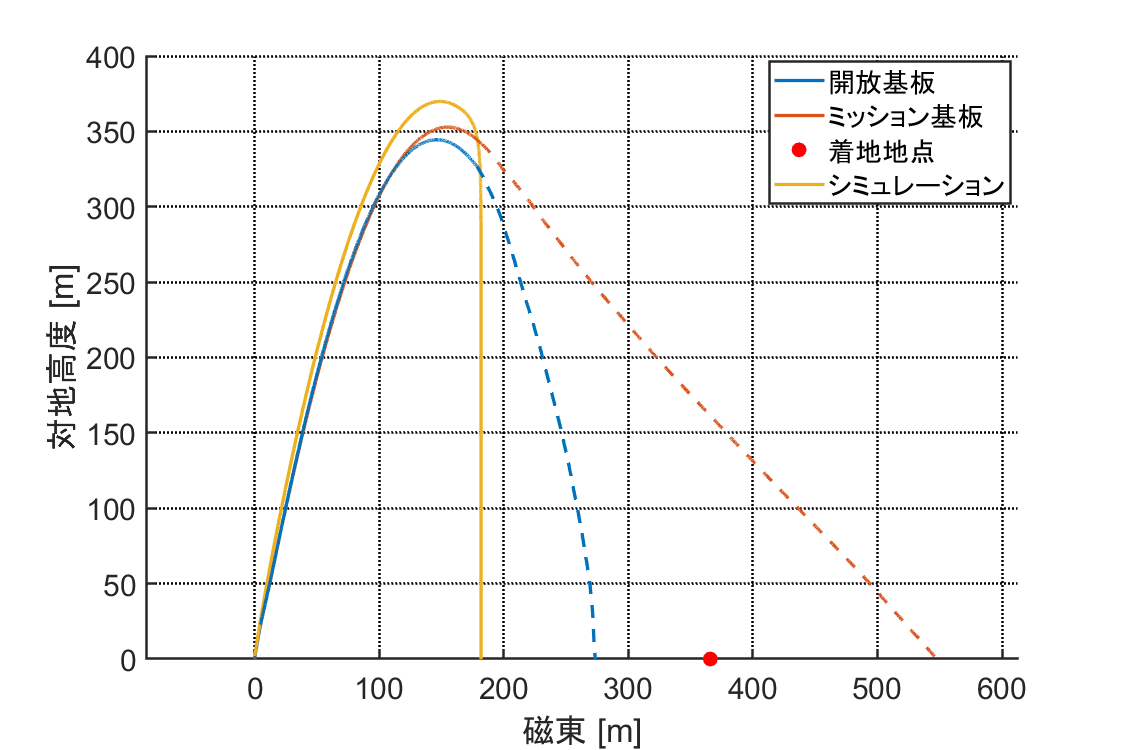
\includegraphics[width=75mm]{pic_sim/pos3_eh.png}
            \hspace{16mm} {\small[1]磁東-対地高度}
        \end{minipage}
        \begin{minipage}{.48\textwidth}
            \centering
            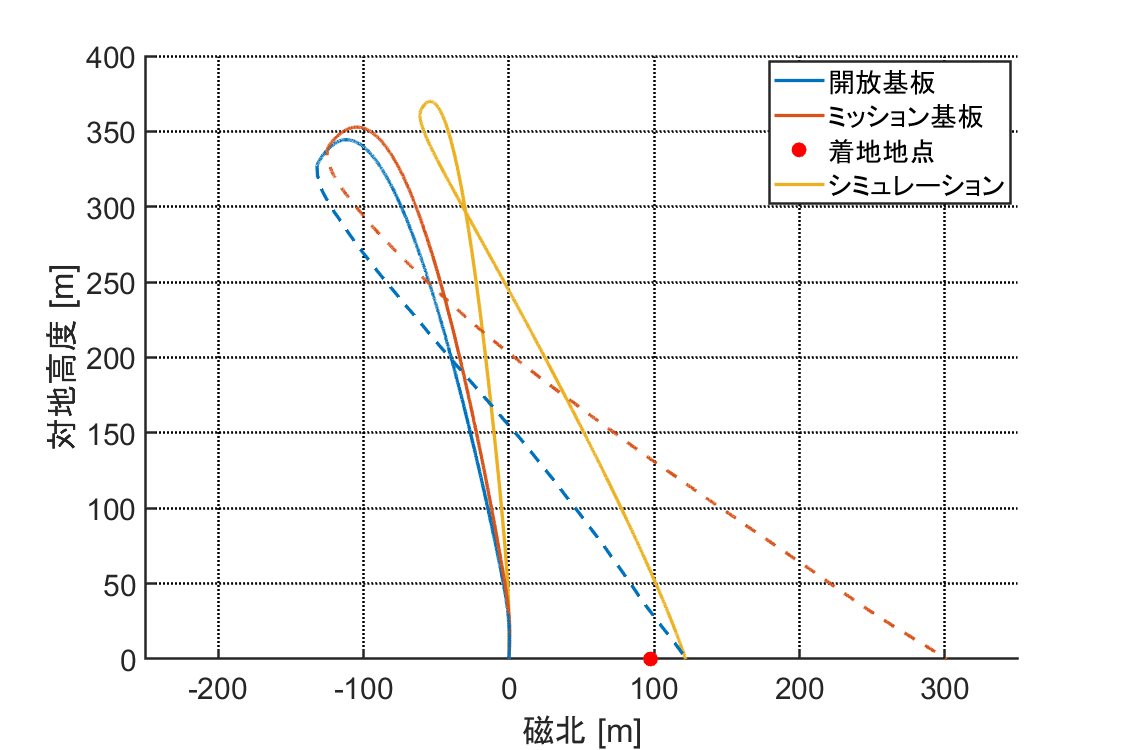
\includegraphics[width=75mm]{pic_sim/pos3_nh.png}
            \hspace{16mm} {\small[2]磁北-対地高度}
        \end{minipage}
    \end{tabular}
    \centering
    \begin{minipage}{.48\textwidth}
        \centering
        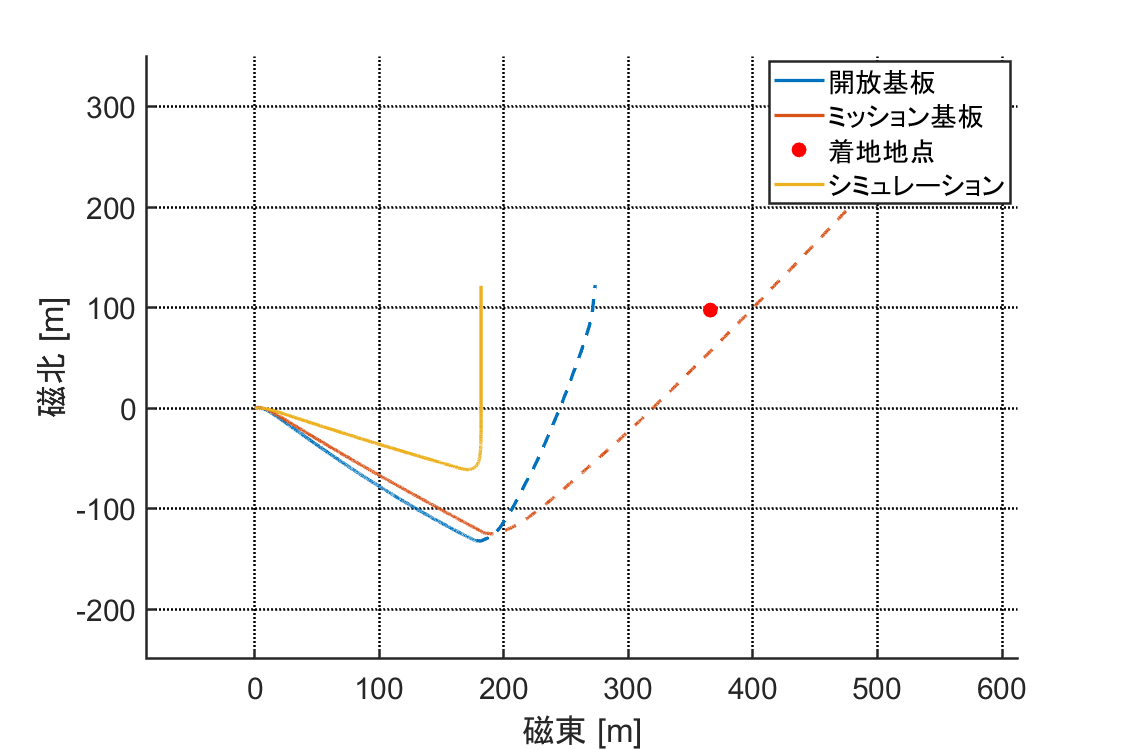
\includegraphics[width=75mm]{pic_sim/pos3_en.png}
        \hspace{16mm}{\small[3]磁東-磁北}
    \end{minipage}
    \caption{飛行経路(風向\SI{180}{deg}風速\SI{3.0}{m/s})}
    \label{fig:hikoukeirosim}
\end{figure}

報告された風向風速条件ではシミュレーションによる落下地点は実際の落下地点から西に約\SI{180}{m}ずれていることが確認できる。
また、最高高度は\ref{koudo}項で示した値より\SI{17}{m}高い結果となった。
これはシミュレーションに使用した推力履歴が7月の燃焼試験でものであり、\ref{suiryokurireki}項で示したように燃焼試験でのトータルインパルスが実際の値より上回っていた事が原因であると考えられる。

さらに、落下地点の差に関しては、風向の違いが大きく関係していると考えられる。
打上げ直前の現地報告では風向が南であったが、推測された飛行経路の開傘地点と実際の落下地点を考慮すると、飛行時の風は南西であったと推測される。
図\ref{fig:hikoukeirosimu225}に南西の風でのシミュレーションの結果示す。


\begin{figure}[H]
    \begin{tabular}{cc}
        \begin{minipage}{.48\textwidth}
            \centering
            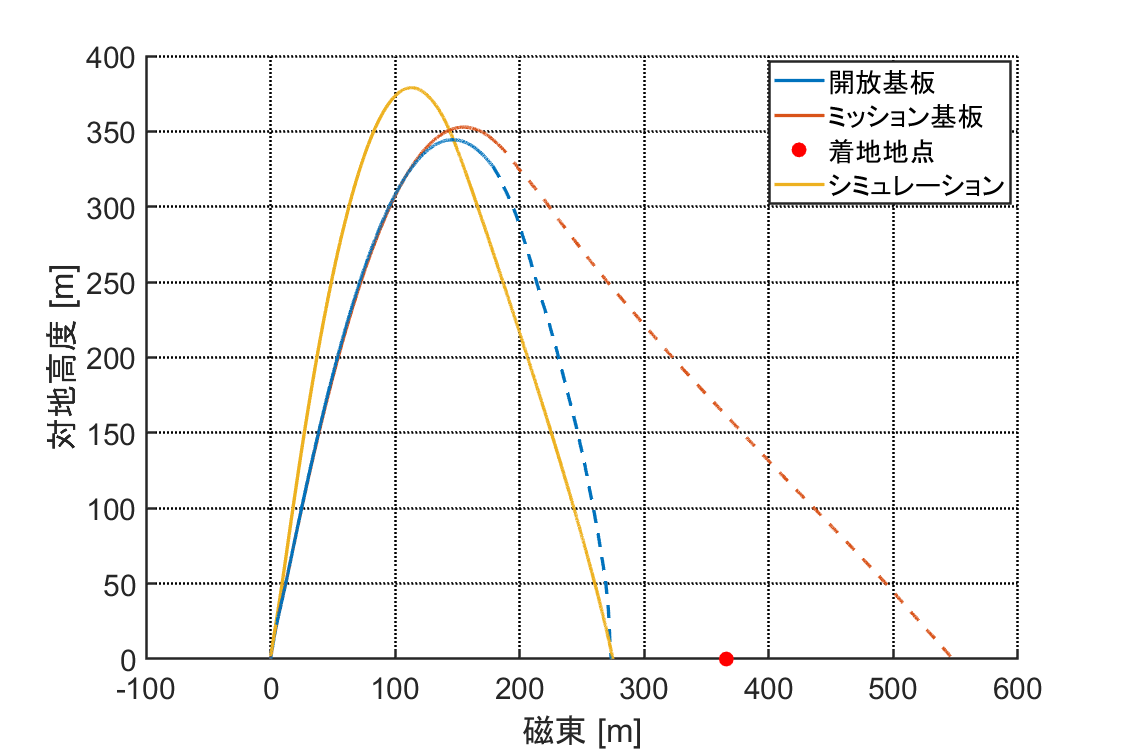
\includegraphics[width=75mm]{pic_sim/pos3_eh_225.png}
            \hspace{16mm} {\small[1]磁東-対地高度}
        \end{minipage}
        \begin{minipage}{.48\textwidth}
            \centering
            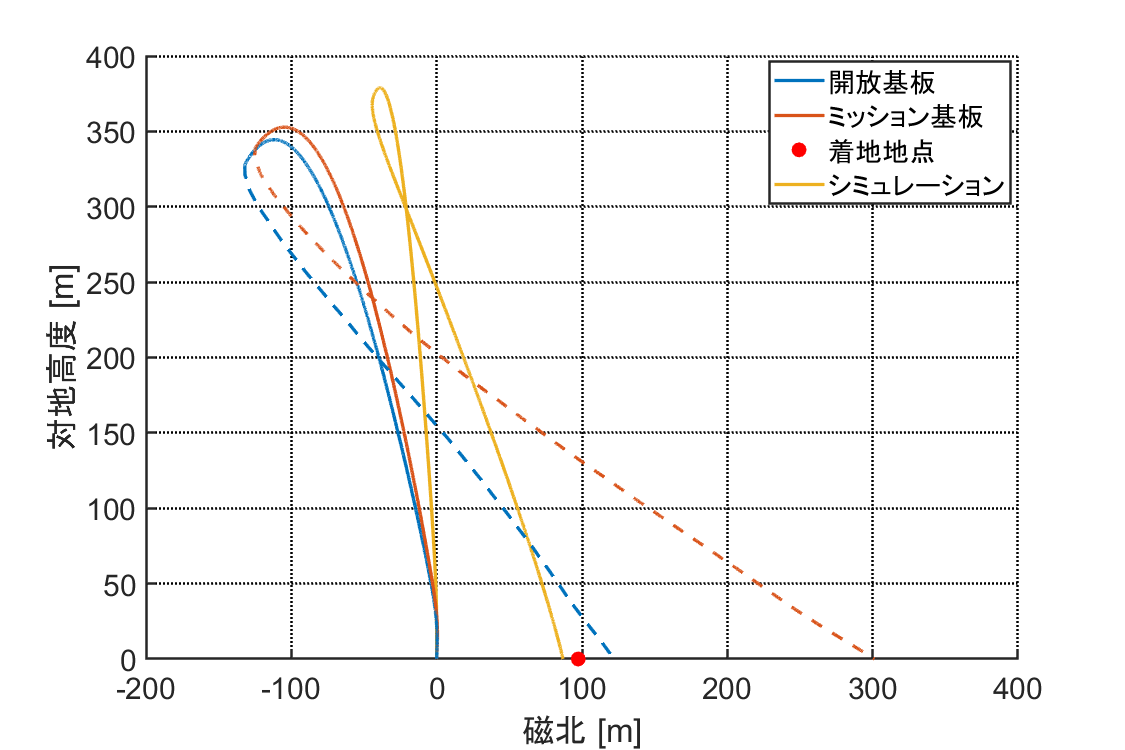
\includegraphics[width=75mm]{pic_sim/pos3_nh_225.png}
            \hspace{16mm} {\small[2]磁北-対地高度}
        \end{minipage}
    \end{tabular}
    \centering
    \begin{minipage}{.48\textwidth}
        \centering
        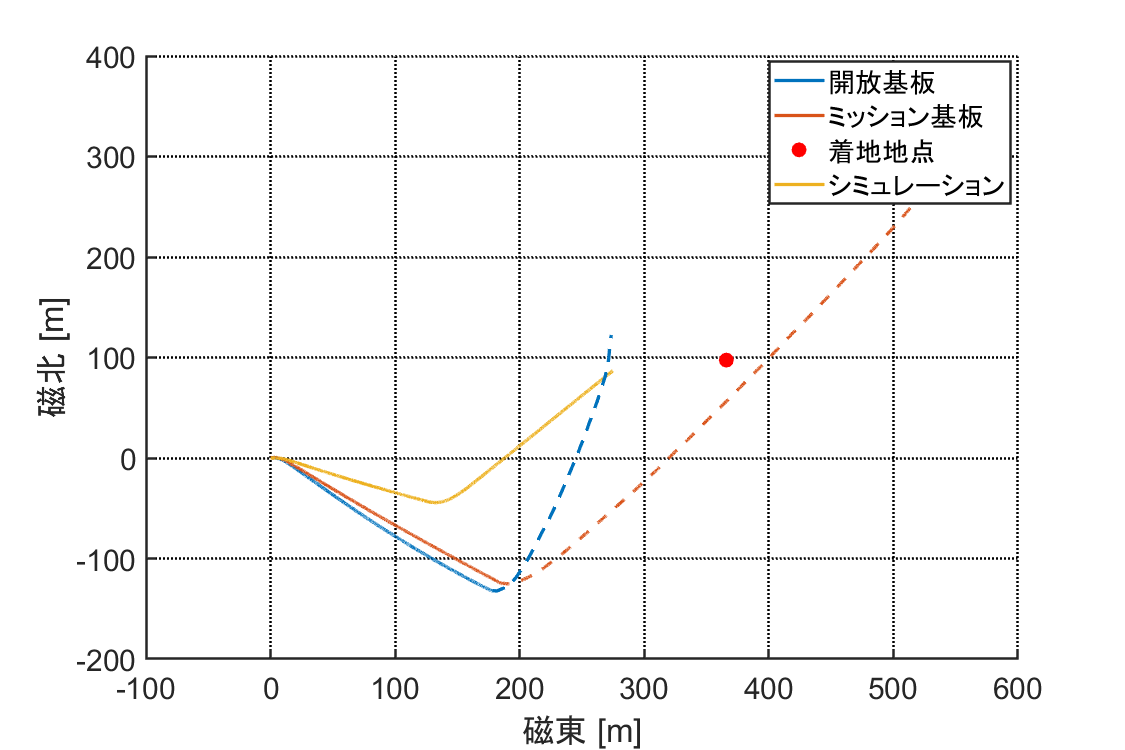
\includegraphics[width=75mm]{pic_sim/pos3_en_225.png}
        \hspace{16mm}{\small[3]磁東-磁北}
    \end{minipage}
    \caption{飛行経路(風向\SI{225}{deg}風速\SI{3.0}{m/s})}
    \label{fig:hikoukeirosimu225}
\end{figure}

結果としては、南風の結果より南西の風でのシミュレーションのほうが落下地点に関しては近くなり、実際の落下地点から西に約\SI{80}{m}であった。


\begin{thebibliography}{99}
    \bibitem{hikourikigaku} 嶋田有三・佐々修一,飛行力学,森北出版株式会社(2017)

\end{thebibliography}

\end{document}
